\documentclass[12pt]{amsart}
\usepackage[T1]{fontenc}
\usepackage[utf8]{inputenc}

\usepackage[top=1.95cm, bottom=1.95cm, left=2.35cm, right=2.35cm]{geometry}

\usepackage{amsmath}
\usepackage{amssymb}
\usepackage{enumitem}
\usepackage{multicol}
\usepackage[french]{babel}
\usepackage[
    type={CC},
    modifier={by-nc-sa},
	version={4.0},
]{doclicense}

\usepackage{tnsmath}

\DeclareMathOperator{\taille}{\tau}

\newtheorem{fact}{Fait}
\newtheorem*{proof*}{Preuve}

\setlength\parindent{0pt}


\newcommand\squote[1]{\og #1 \fg{}}


\begin{document}

\title{BROUILLON - CANDIDAT - À propos de l'exercice de SPÉ MATHS du BAC S de Juin 2018 (Métropole)}
\author{Christophe BAL}
\date{25 Juin 2018 - 26 Juillet 2019}
\maketitle


\begin{center}
	\itshape
	Document, avec son source \LaTeX, disponible sur la page
	
	\url{https://github.com/bc-writing/drafts}.
\end{center}


\bigskip


\begin{center}
	\hrule\vspace{.3em}
	{
		\fontsize{1.35em}{1em}\selectfont
		\textbf{Mentions \og légales \fg}
	}
			
	\vspace{0.45em}
	\doclicenseThis
	\hrule
\end{center}



\setcounter{tocdepth}{2}
\tableofcontents



\section{Ce qui interroge : une matrice \squote{magique} sortie d'un chapeau}

Dans le BAC S de Juin 2018 (Métropole), la partie A de l'exercice de Spécialité Mathématiques s'intéressait à l'équation diophantienne \textbf{[ED]} : $x^2 - 8 y^2 = 1$ sur $\NN^2$.


\medskip

On a une solution évidente $(x \,; y) = (3 \,; 1)$ puis l'exercice introduit une matrice \squote{magique}
$A =
\begin{pmatrix} 
  3 & 8  \\ 
  1 & 3 
\end{pmatrix}$
pour ensuite construite des solutions $(x_n \,; y_n)$ de façon récursive et linéaire comme suit :
$\begin{pmatrix} 
  x_{n+1} \\ 
  y_{n+1} 
\end{pmatrix}
=
A
\begin{pmatrix} 
  x_{n} \\ 
  y_{n} 
\end{pmatrix}
$ .


\medskip

Très bien mais mais comment peut-on découvrir la matrice \squote{magique} $A$ ?



\section{Un moyen élémentaire de découvrir la matrice \squote{magique}}

Une idée élémentaire pour découvrir la matrice \squote{magique} $A$ est de noter que nous pouvons écrire
$x^2 - 8 y^2
=
\begin{pmatrix} 
  x & y 
\end{pmatrix}
Q
\begin{pmatrix} 
  x \\ 
  y 
\end{pmatrix}$
en posant
$Q
=
\begin{pmatrix} 
  1 & 0  \\ 
  0 & -8 
\end{pmatrix}$ 
\textit{
	(le lecteur connaissant les formes quadratiques ne sera pas surpris par cette réécriture) 
}.


\medskip

En posant 
$\begin{pmatrix} 
  X \\ 
  Y 
\end{pmatrix}
=
A
\begin{pmatrix} 
  x \\ 
  y 
\end{pmatrix}$ ,
comme nous avons
$\begin{pmatrix} 
  X & Y 
\end{pmatrix}
Q
\begin{pmatrix} 
  X \\ 
  Y 
\end{pmatrix}
=
\begin{pmatrix} 
  x & y 
\end{pmatrix}
A^T Q A
\begin{pmatrix} 
  x \\ 
  y 
\end{pmatrix}$ ,
il est alors naturel de chercher $A$ vérifiant $A^T Q A = Q$ car d'une solution
$\begin{pmatrix} 
  x \\ 
  y 
\end{pmatrix}$
on pourra passer à une \squote{autre} solution
$\begin{pmatrix} 
  X \\ 
  Y 
\end{pmatrix}
=
A \begin{pmatrix} 
  x \\ 
  y 
\end{pmatrix}$
comme dans le sujet du BAC S.


\bigskip

Utilisant le déterminant, nous avons comme contrainte immédiate que $\det A = \pm 1$ \textit{($A$ doit donc être inversible)}. 


% ------------------ %


\bigskip

\textit{\textbf{Cas 1 :} supposons d'abord que $\det A = 1$ .}

\medskip

Notant
$A = \begin{pmatrix} 
  a & b \\ 
  c & d
\end{pmatrix}$ ,
nous avons alors
$A^{-1} = \begin{pmatrix} 
  d  & -b \\ 
  -c & a
\end{pmatrix}$
d'où :

\begin{flalign*}
	A^T Q A = Q & \Longleftrightarrow  A^T Q = Q A^{-1} & \\
	            & \Longleftrightarrow 
	\begin{pmatrix} 
	  a & c \\ 
	  b & d
	\end{pmatrix}
	\begin{pmatrix} 
	  1 & 0  \\ 
	  0 & -8 
	\end{pmatrix}
	=
	\begin{pmatrix} 
	  1 & 0  \\ 
	  0 & -8 
	\end{pmatrix}
	\begin{pmatrix} 
	  d  & -b \\ 
	  -c & a
	\end{pmatrix}
	                                                    & \\
	            & \Longleftrightarrow 
	\begin{pmatrix} 
	  a & -8 c \\ 
	  b & -8 d
	\end{pmatrix}
	=
	\begin{pmatrix} 
	  d  & -b \\ 
	  8c & -8a
	\end{pmatrix}
	                                                    & \\
	            & \Longleftrightarrow a = d \text{ et } b = 8c 
\end{flalign*}


\medskip

La condition $\det A = 1$ pour
$A
=
\begin{pmatrix} 
  a & b \\ 
  c & d
\end{pmatrix}
=
\begin{pmatrix} 
  a & 8c \\ 
  c & a
\end{pmatrix}$
nous donne
$a^2 - 8c^2 = 1$ . Que c'est joli !


\medskip

Notons que l'ensemble des matrices de ce type est stable par multiplication, et que la matrice du sujet de BAC n'est autre que celle correspondant à la solution élémentaire
$(a \,; c) = (3 \,; 1)$.


% ------------------ %


\bigskip

\textit{\textbf{Cas 2 :} supposons maintenant que $\det A = -1$ .}

\medskip

Notant
$A = \begin{pmatrix} 
  a & b \\ 
  c & d
\end{pmatrix}$ ,
nous avons alors
$A^{-1} = \begin{pmatrix} 
  -d & b  \\ 
   c & -a
\end{pmatrix}$
d'où comme dans les calculs précédents :
$A^T Q A = Q \Longleftrightarrow a = -d \text{ et } b = -8c$ .


\bigskip

La condition $\det A = -1$ pour
$A
=
\begin{pmatrix} 
  a & b \\ 
  c & d
\end{pmatrix}
=
\begin{pmatrix} 
  a & -8c \\ 
  c & -a
\end{pmatrix}$
nous redonne
$a^2 - 8c^2 = 1$ mais avec un autre ensemble de matrices qui lui n'est pas stable par multiplication.





\section{Prenons un peu de hauteur : un groupe \squote{caché}}

Ce qui suit reprend les excellentes indications données par Jérôme Germoni dans une discussion au bas de cette page :
\url{http://images.math.cnrs.fr/+Nombres-puissants-au-bac-S+}
\textit{(chercher les messages de l'utilisateur projetmbc)}.


\bigskip

Dans la suite, nous ne considérons que l'ensemble des matrices $A$ telles que $A^T Q A = Q$ et $\det A = 1$ afin de pouvoir les multiplier entre elles.


\medskip

Nous savons que $A$ est du type 
$A
=
\begin{pmatrix} 
  a & 8c \\ 
  c & a
\end{pmatrix}$ 
et que la contrainte $a^2 - 8c^2 = 1$ est cachée dans la relation $A^T Q A = Q$ .


\medskip

Nous savons aussi que si
$\begin{pmatrix} 
  x \\ 
  y 
\end{pmatrix}$
verifie $x^2 - 8 y^2 = 1$ , il en sera de même pour
$\begin{pmatrix} 
  X \\ 
  Y 
\end{pmatrix}
=
A
\begin{pmatrix} 
  x \\ 
  y 
\end{pmatrix}$
où
$\begin{pmatrix} 
  X \\ 
  Y 
\end{pmatrix}
=
\begin{pmatrix} 
  a x + 8c y \\ 
  c x + a y
\end{pmatrix}$ .


\medskip

Notant $\setproba{S}$ l'ensemble des solutions entières
\footnote{
	Ce qui suit se généralise aux solutions rationnelles, à celles réelles ou encore à celles complexes mais ne sortons pas du cadre de ce modeste document.
}
de \textbf{[ED]} : $x^2 - 8 y^2 = 1$ , ce qui précède motive la définition de la loi $\star$ sur $\setproba{S}$ via
$\begin{pmatrix} 
  a \\ 
  c 
\end{pmatrix}
\star
\begin{pmatrix} 
  x \\ 
  y 
\end{pmatrix}
=
\begin{pmatrix} 
  a x + 8c y \\ 
  c x + a y
\end{pmatrix}$ .
Nous allons démontrer que cette loi $\star$ est bien définie et qu'elle fait de $\setproba{S}$ un groupe. Très joli ! Non ?


\medskip

Les raisonnements suivants se font en faisant le parallèle entre 
$\begin{pmatrix} 
  a \\ 
  c 
\end{pmatrix}
\star
\begin{pmatrix} 
  x \\ 
  y 
\end{pmatrix}$
et la matrice produit
$\begin{pmatrix} 
  a & 8c \\ 
  c & a 
\end{pmatrix}
\begin{pmatrix} 
  x & 8y \\ 
  y & x 
\end{pmatrix}$
dont on garde juste la première colonne
\footnote{
	Les résultats présentés ici se vérifient et se trouvent directement à la main sans passer par les matrices mais ceci est bien moins élégant.
} .
Rappelons que les deux matrices du produit précédent sont des matrices entières $A$ vérifiant $A^T Q A = Q$ et $\det A = 1$ . Nous savons que pour ce type de matrice la première colonne est solution de \textbf{[ED]} .


\begin{itemize}[label=\small\textbullet]
	\item La loi $\star$ est bien interne à $\setproba{S}$ car si $A^T Q A = Q$ avec $\det A = 1$ et $B^T Q B = Q$ avec $\det B = 1$ , alors nous avons :
	
	\begin{itemize}[label=\raisebox{.3ex}{$\centerdot$}]
		\item $(AB)^T Q (AB) = B^T A^T Q A B = B^T Q B = Q$
		
		\medskip
		\item $\det(AB) = \det A \cdot \det B = 1$
	\end{itemize}


	\medskip
	\item
	$\begin{pmatrix} 
	  1 \\ 
	  0 
	\end{pmatrix}$
	est l'élément neutre de $\star$ car sa matrice associée est la matrice identité.


	\medskip
	\item
	$\begin{pmatrix} 
	  a  \\ 
	  -c 
	\end{pmatrix}$
	est l'inverse de
	$\begin{pmatrix} 
	  a \\ 
	  c 
	\end{pmatrix}$
	\textit{(revoir si besoin le cas 1 de la section précédente)}.


	\medskip
	\item Pour finir, l'associativité de $\star$ découle de celle de la multiplication des matrices.
\end{itemize}




\section{Tout est géométrie... Ou presque}

Ce qui suit tente de donner une explication naturelle du lien entre la loi $\star$ et un procédé géométrique rappelé par Jérôme Germoni précédemment cité.


\bigskip

Jusqu'à présent, nous n'avons à aucun moment représenter l'hyperbole $\setgeo{H}$ \squote{à deux branches} d'équation implicite $X^2 - 8 Y^2 = 1$ \textit{(on utilise ici des majuscules pour le système de coordonnées)}. C'est un peu dommage !


\medskip

Ci-dessous se trouvent quatre représentations avec deux points $M$ et $N$ sur $\setgeo{H}$ de coordonnées respectives 
$\begin{pmatrix}
  x \\ 
  y 
\end{pmatrix}$
et
$\begin{pmatrix} 
  x' \\ 
  y' 
\end{pmatrix}$
ainsi que les points $E$ , cf. le neutre de $\star$ , et $P$, eux aussi sur $\setgeo{H}$ , de coordonnées respectives 
$\begin{pmatrix}
  1 \\ 
  0 
\end{pmatrix}$
et
$\begin{pmatrix} 
  x'' \\ 
  y''
\end{pmatrix}
=
\begin{pmatrix}
  x \\ 
  y 
\end{pmatrix}
\star
\begin{pmatrix} 
  x' \\ 
  y'
\end{pmatrix}
=
\begin{pmatrix}
  x x' + 8 y y' \\ 
  x y' + x' y 
\end{pmatrix}$ .


\bigskip


\begin{multicols}{2}
	\center
	
	\fbox{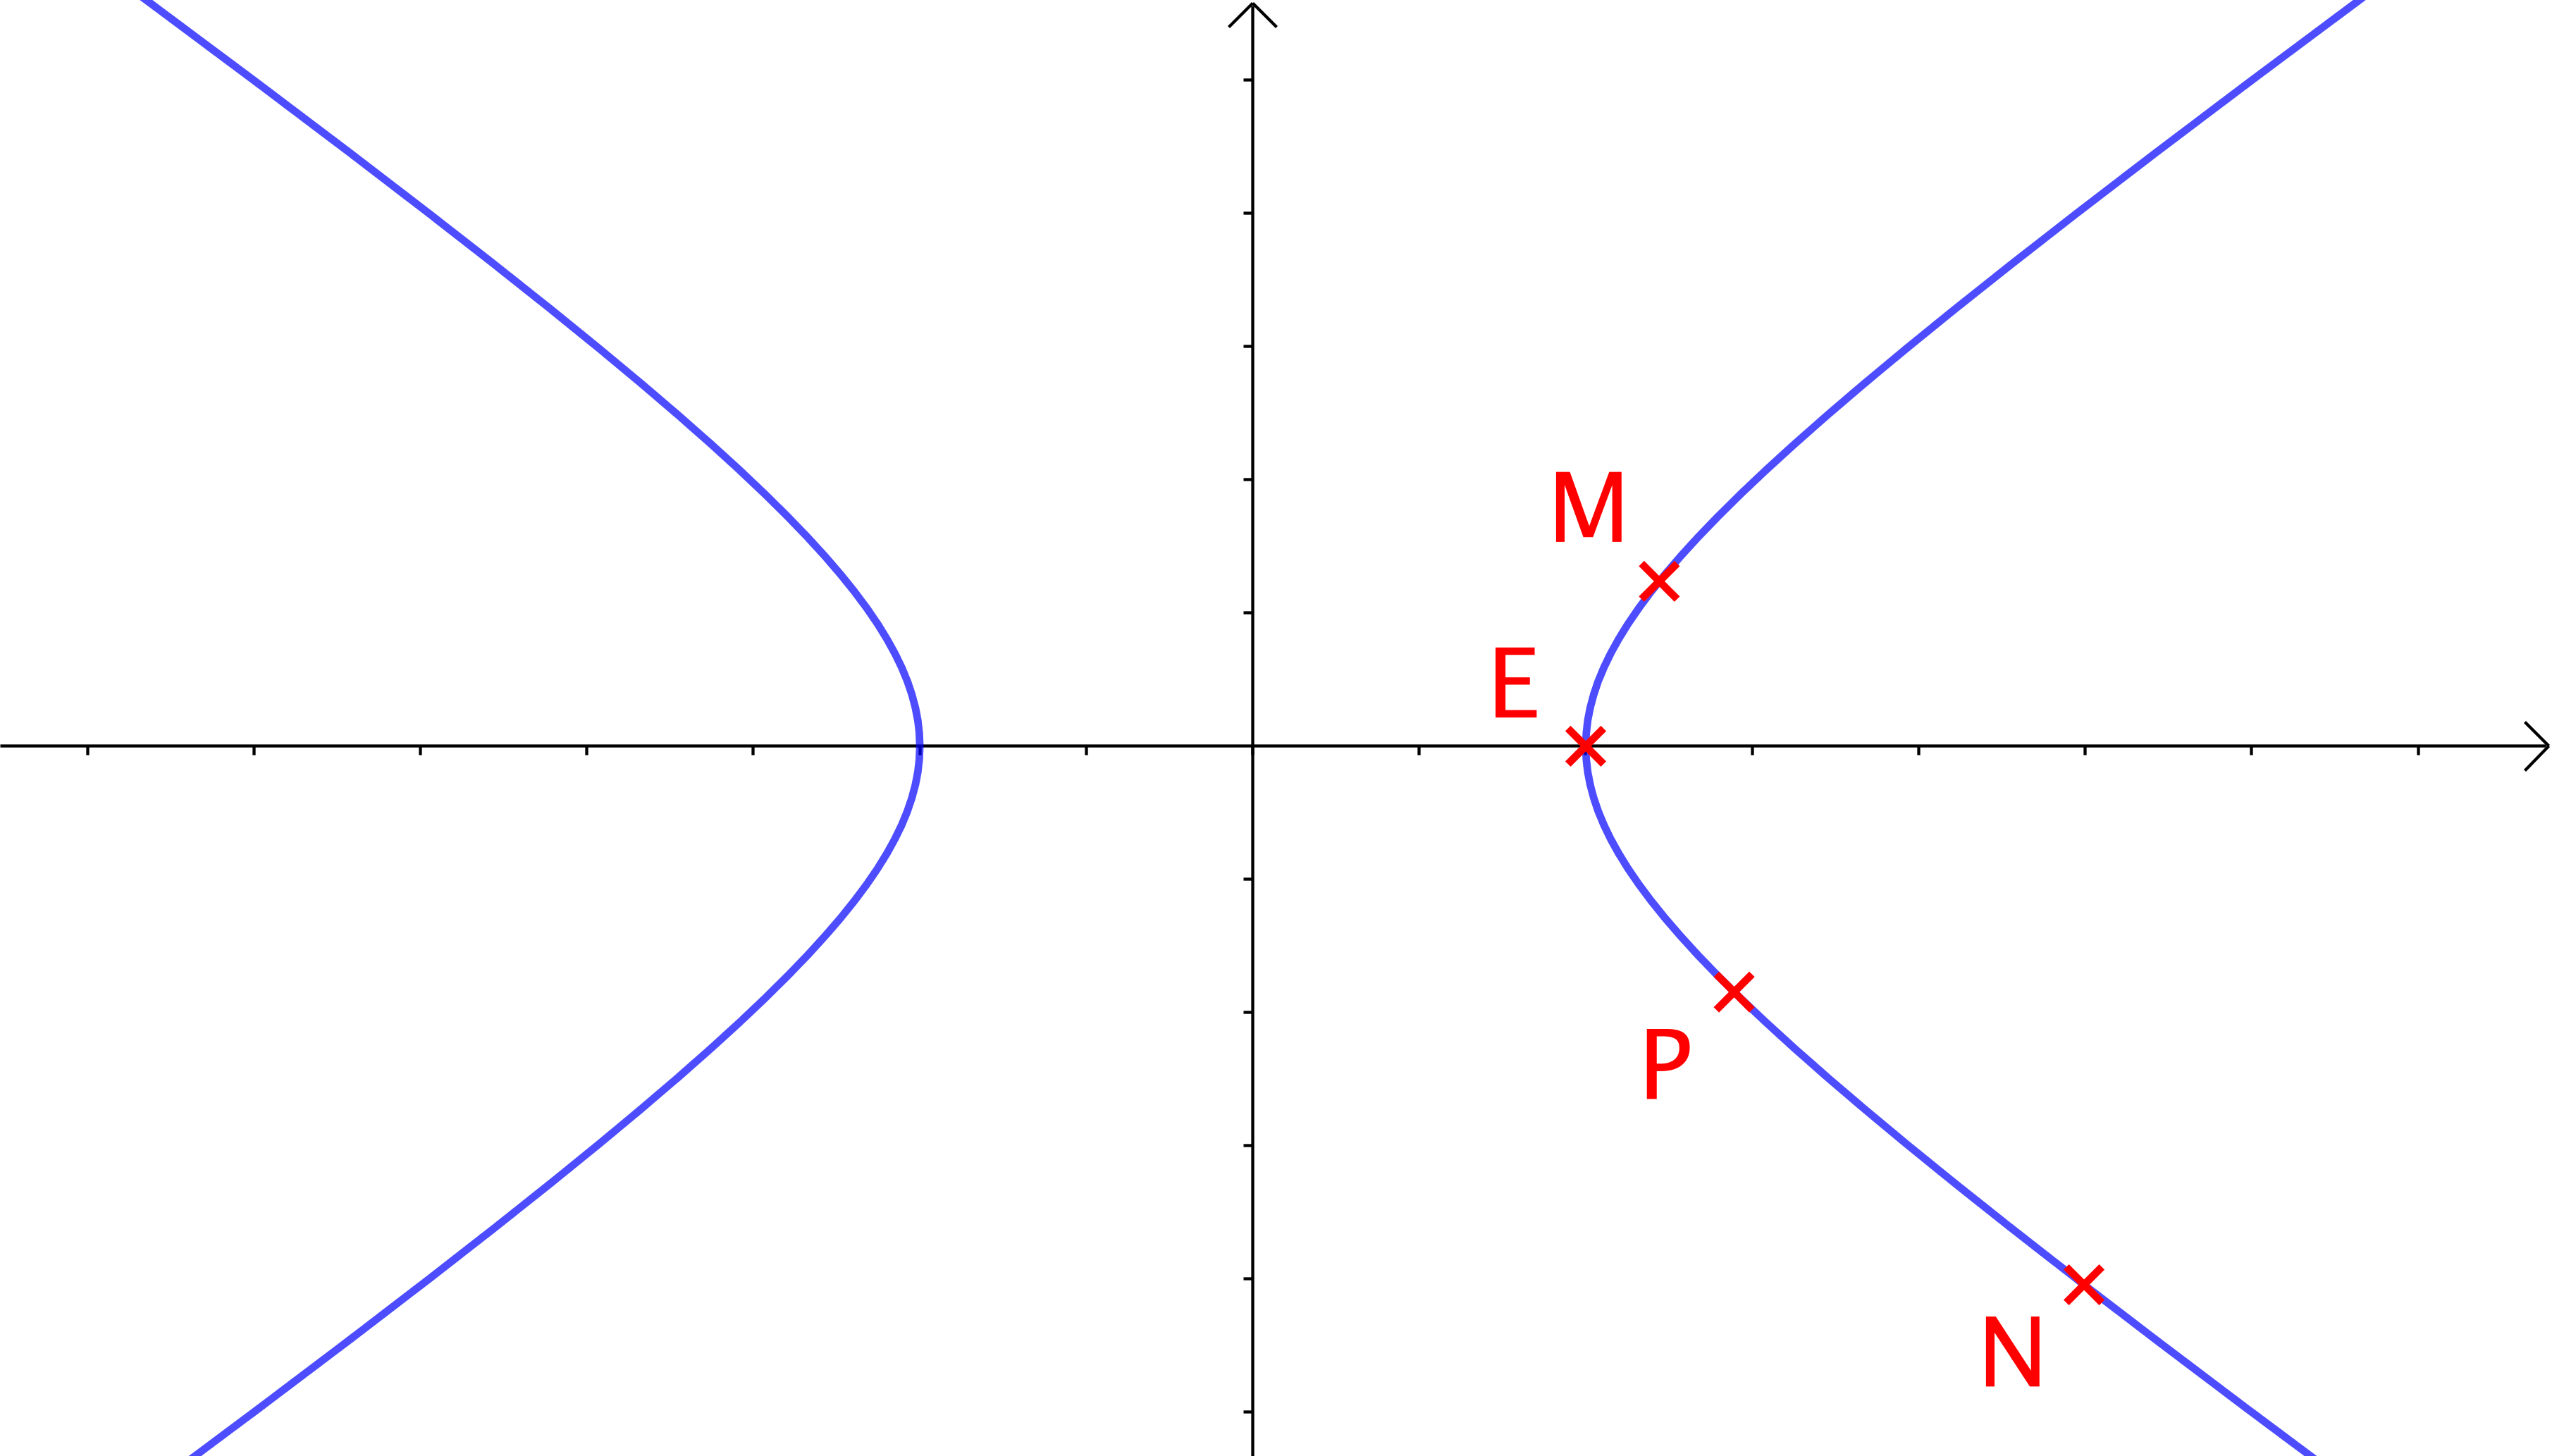
\includegraphics[scale = .5]{exo-spe-math-bac-s-juin-2018/geometry-is-the-queen/oblic-1.png}}
	
	\bigskip
	
	\fbox{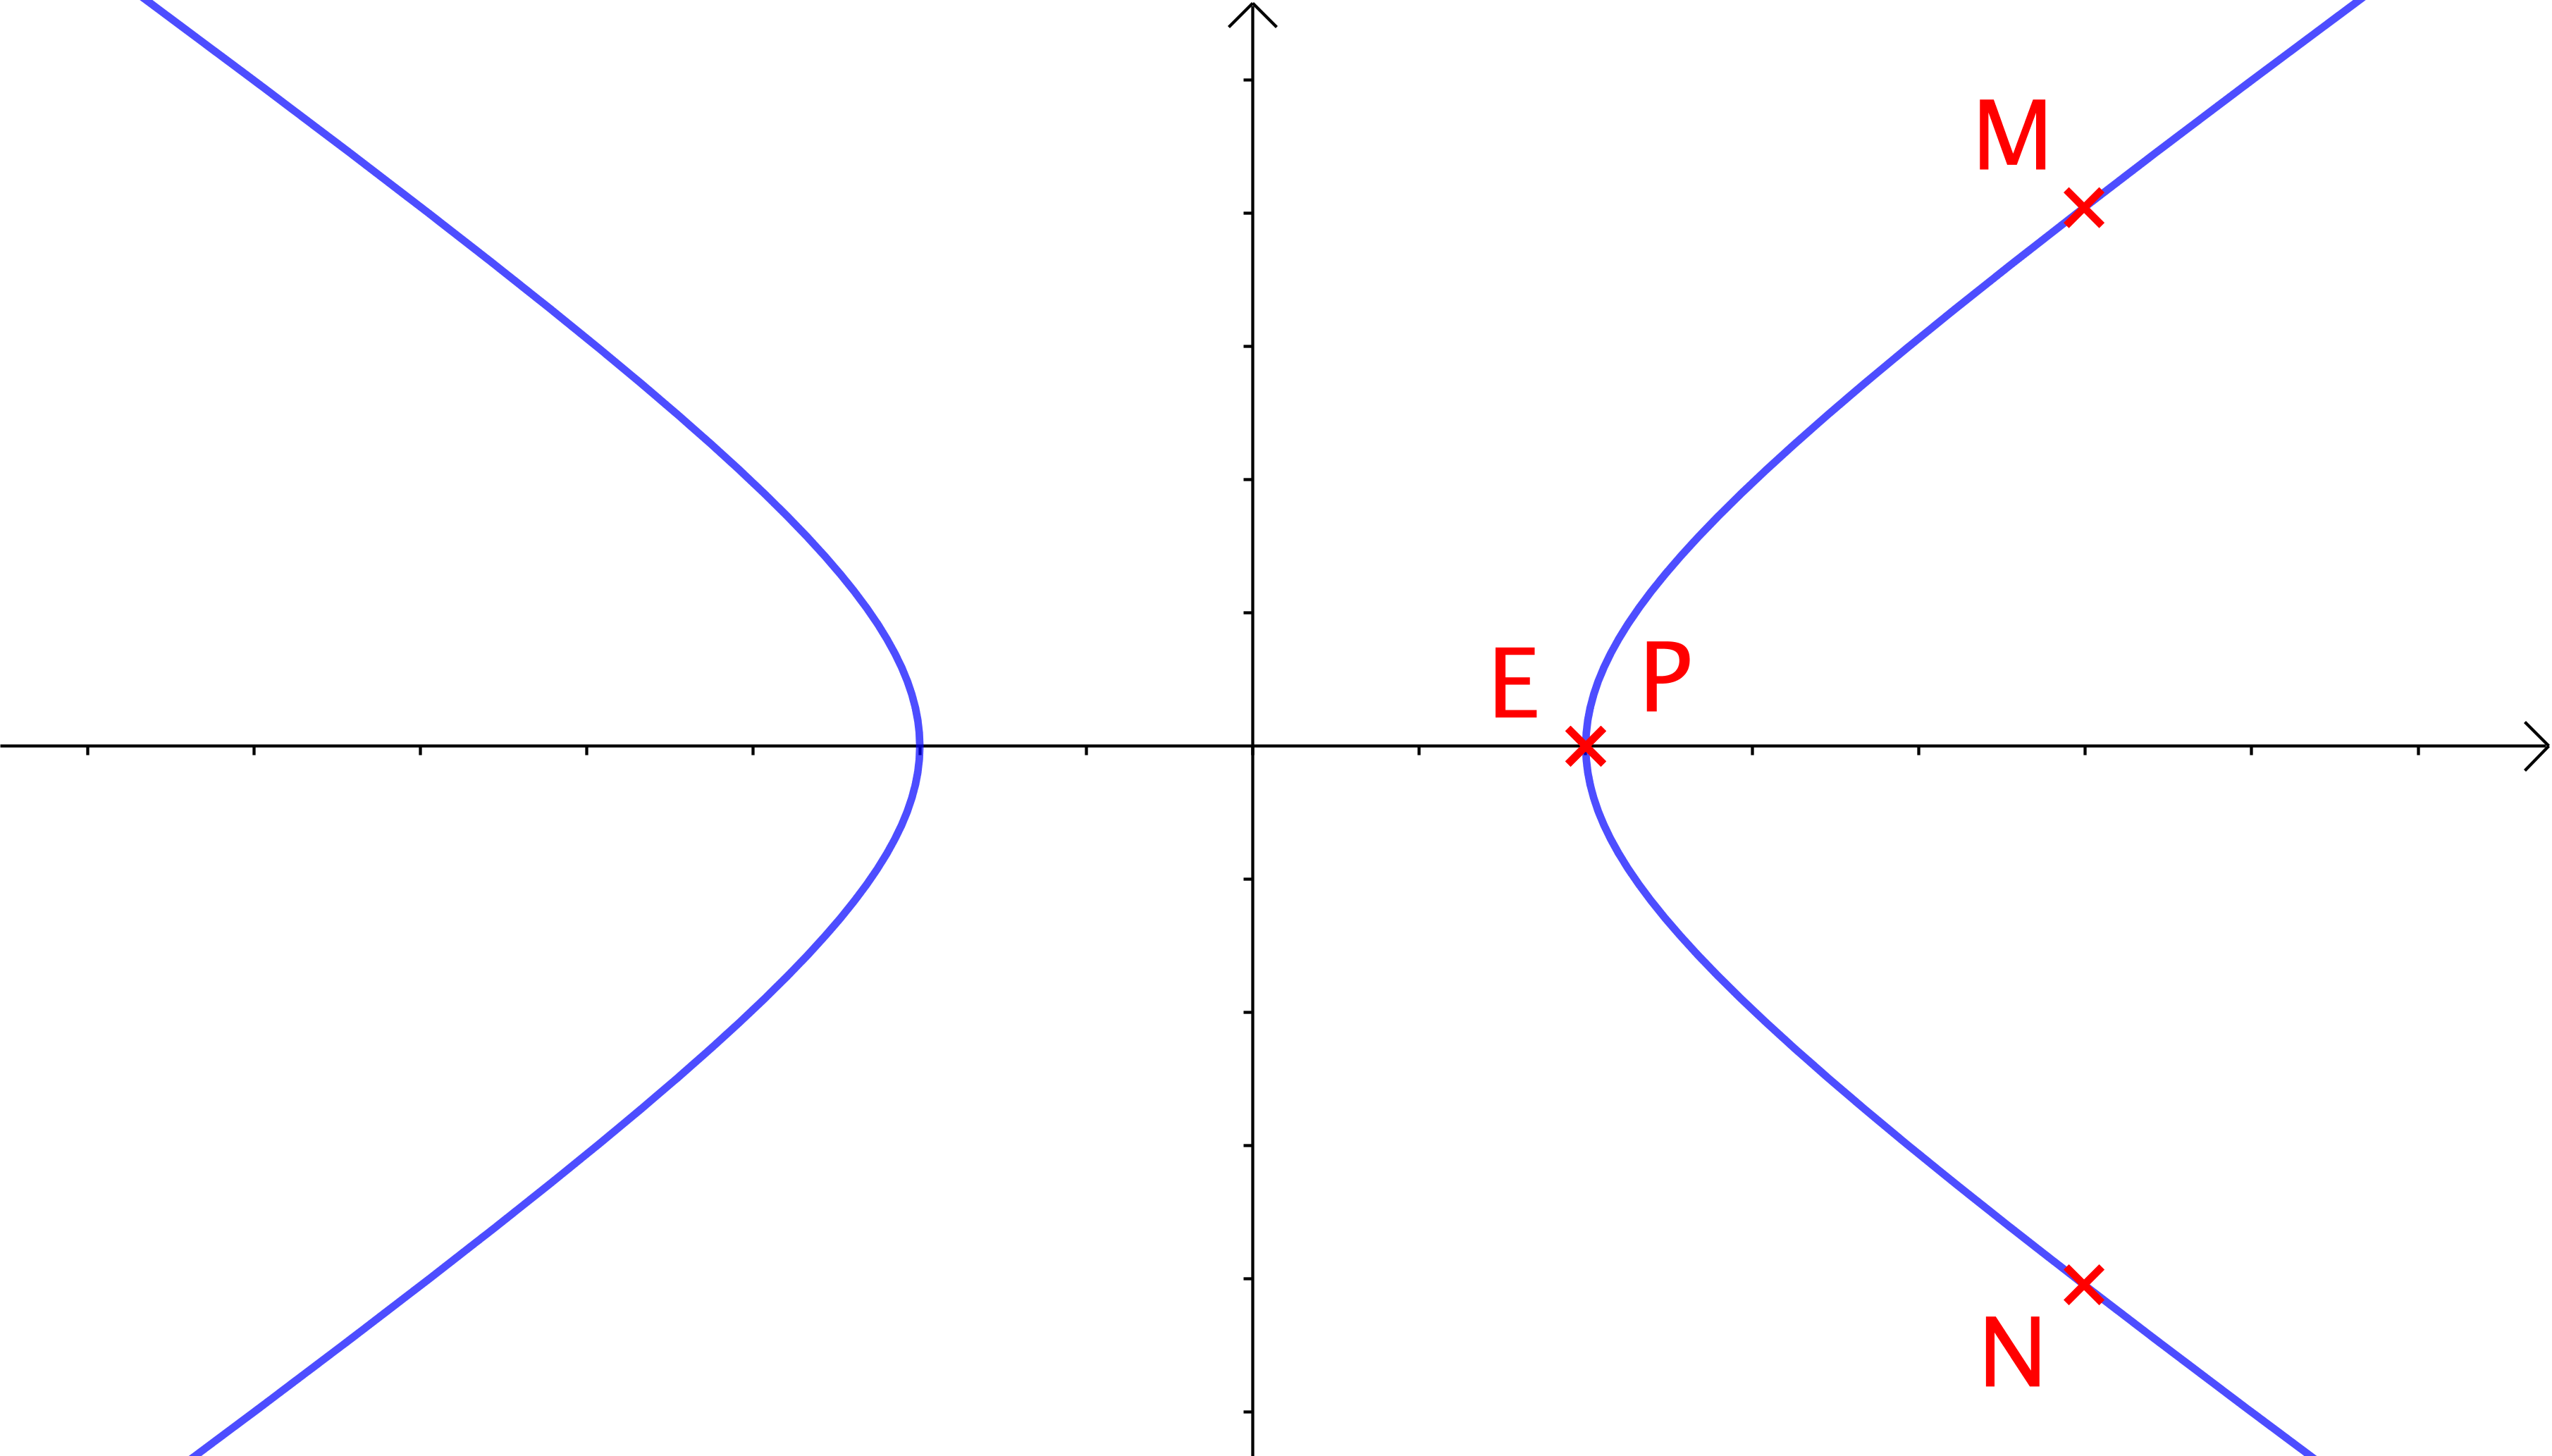
\includegraphics[scale = .5]{exo-spe-math-bac-s-juin-2018/geometry-is-the-queen/vertical-case.png}}

	\columnbreak
	
	\fbox{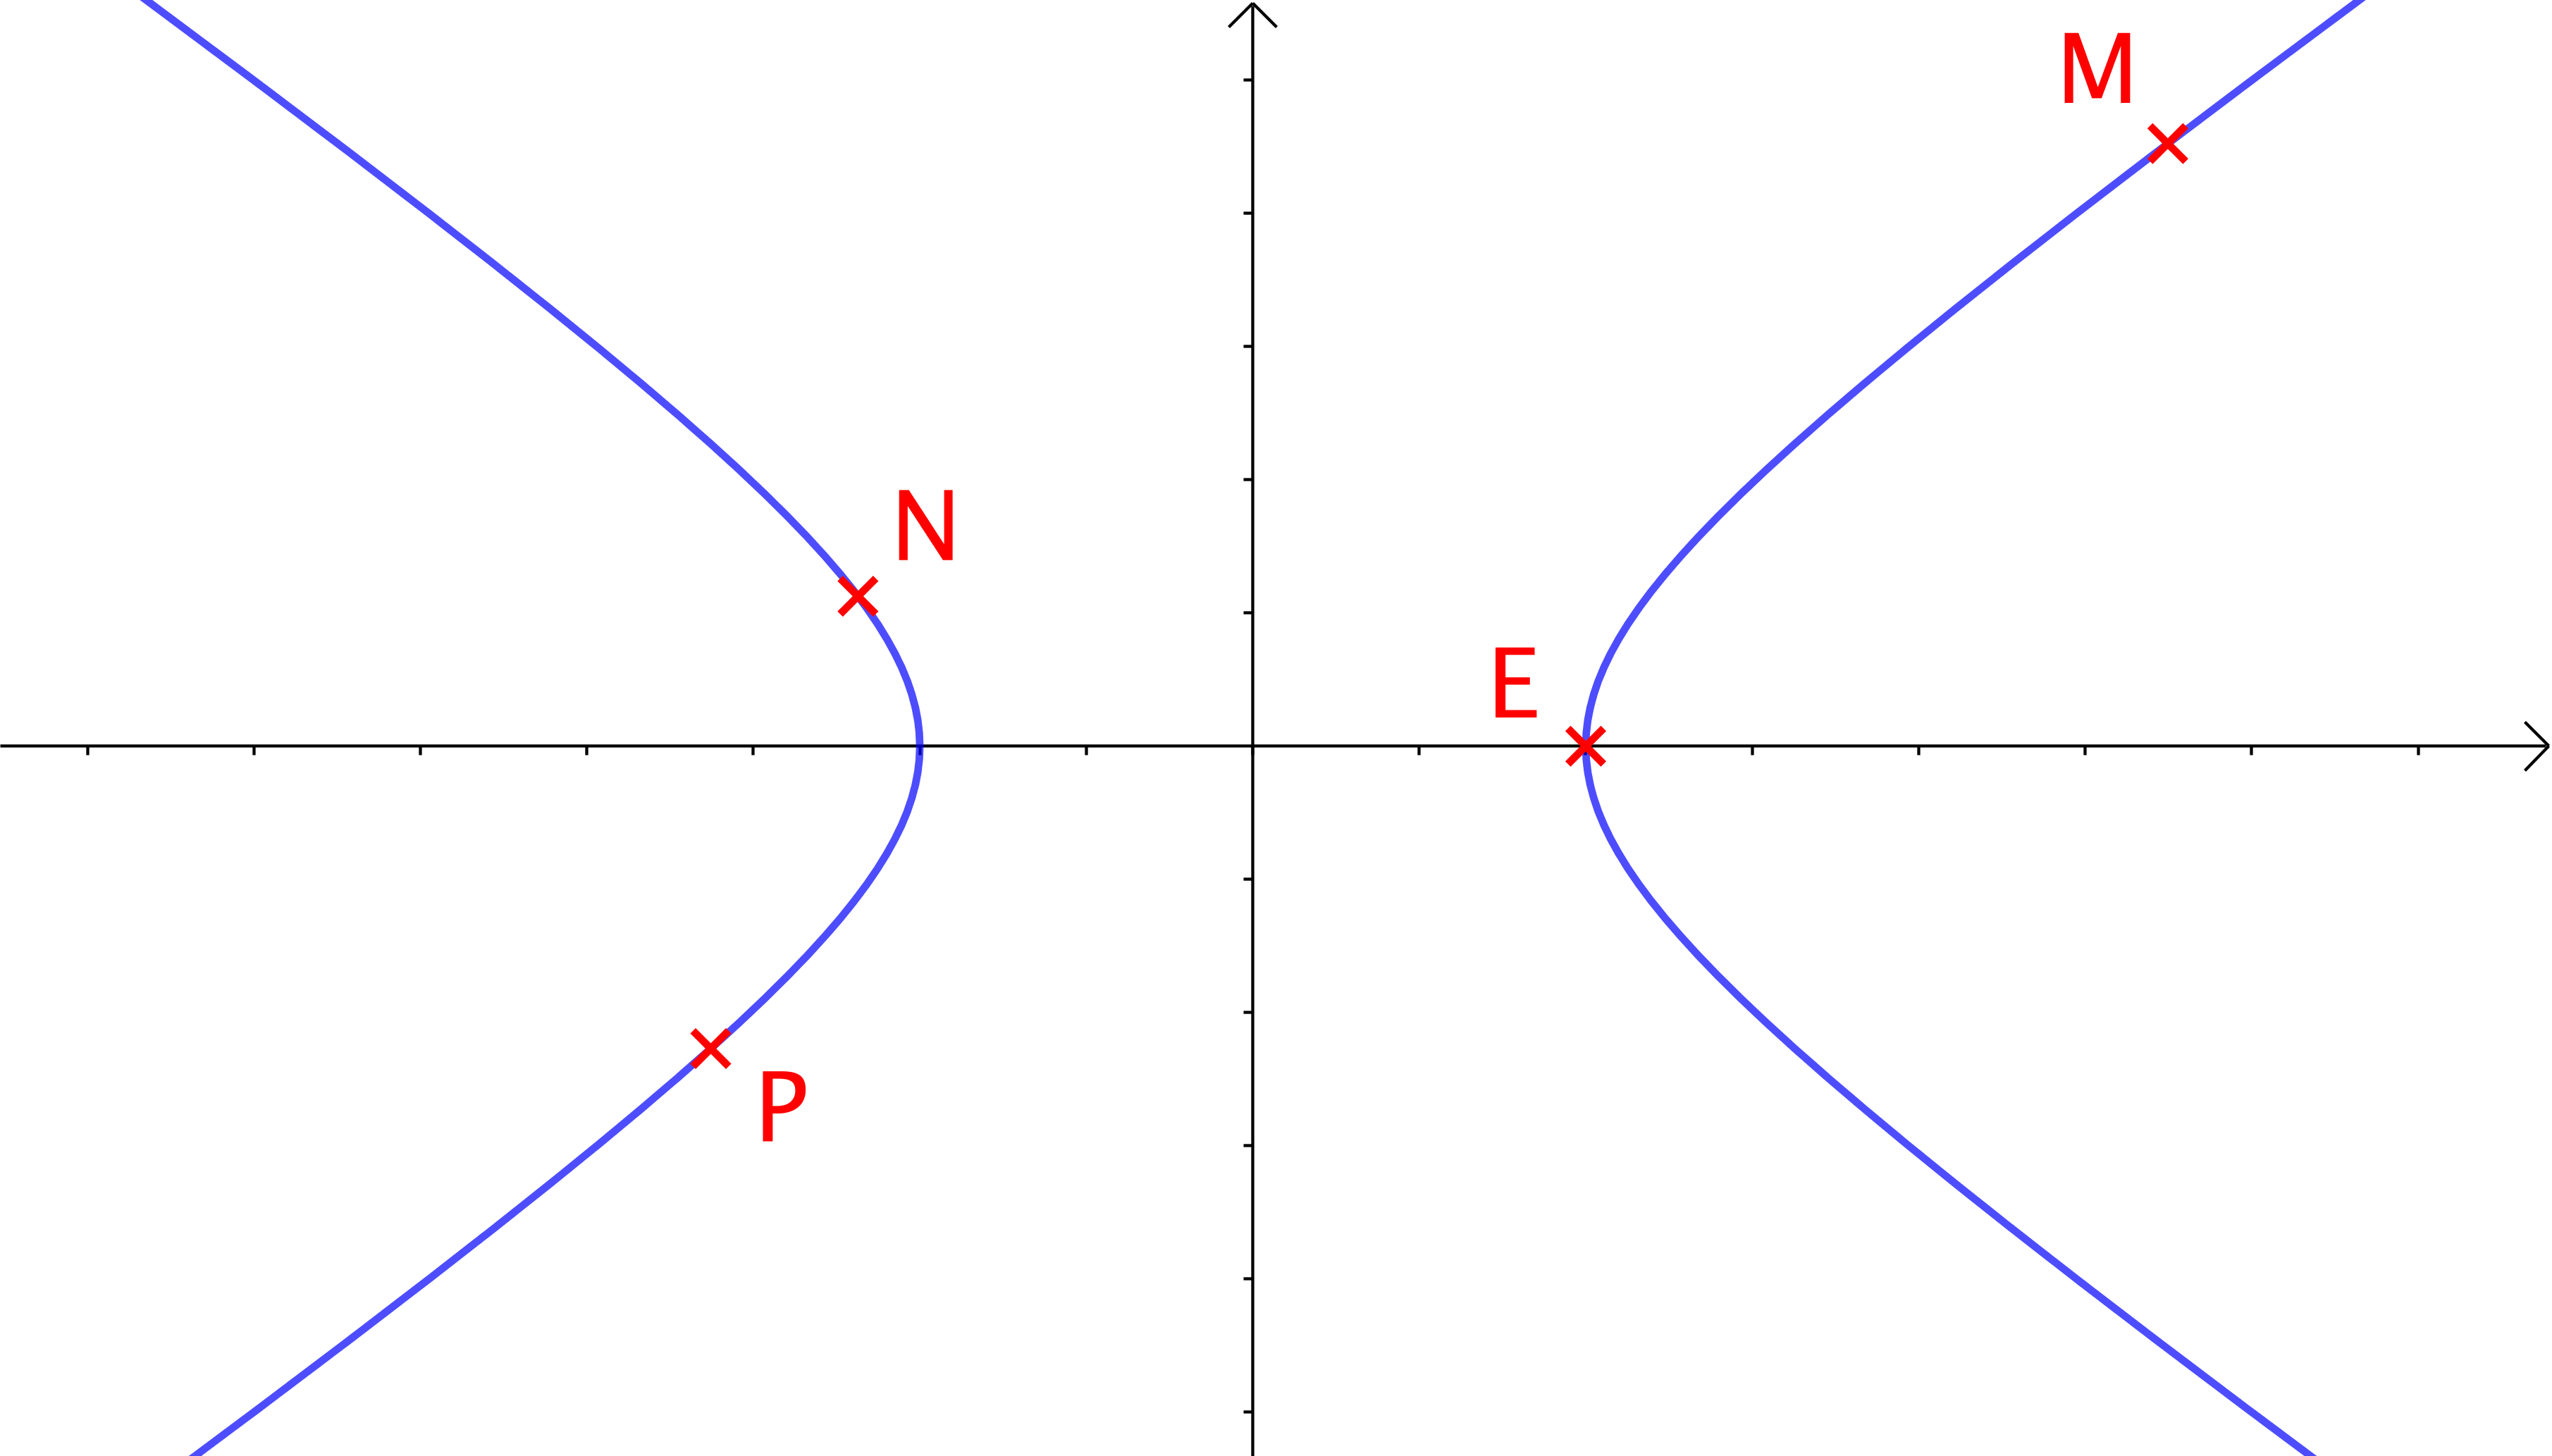
\includegraphics[scale = .5]{exo-spe-math-bac-s-juin-2018/geometry-is-the-queen/oblic-2.png}}
	
	\bigskip

	\fbox{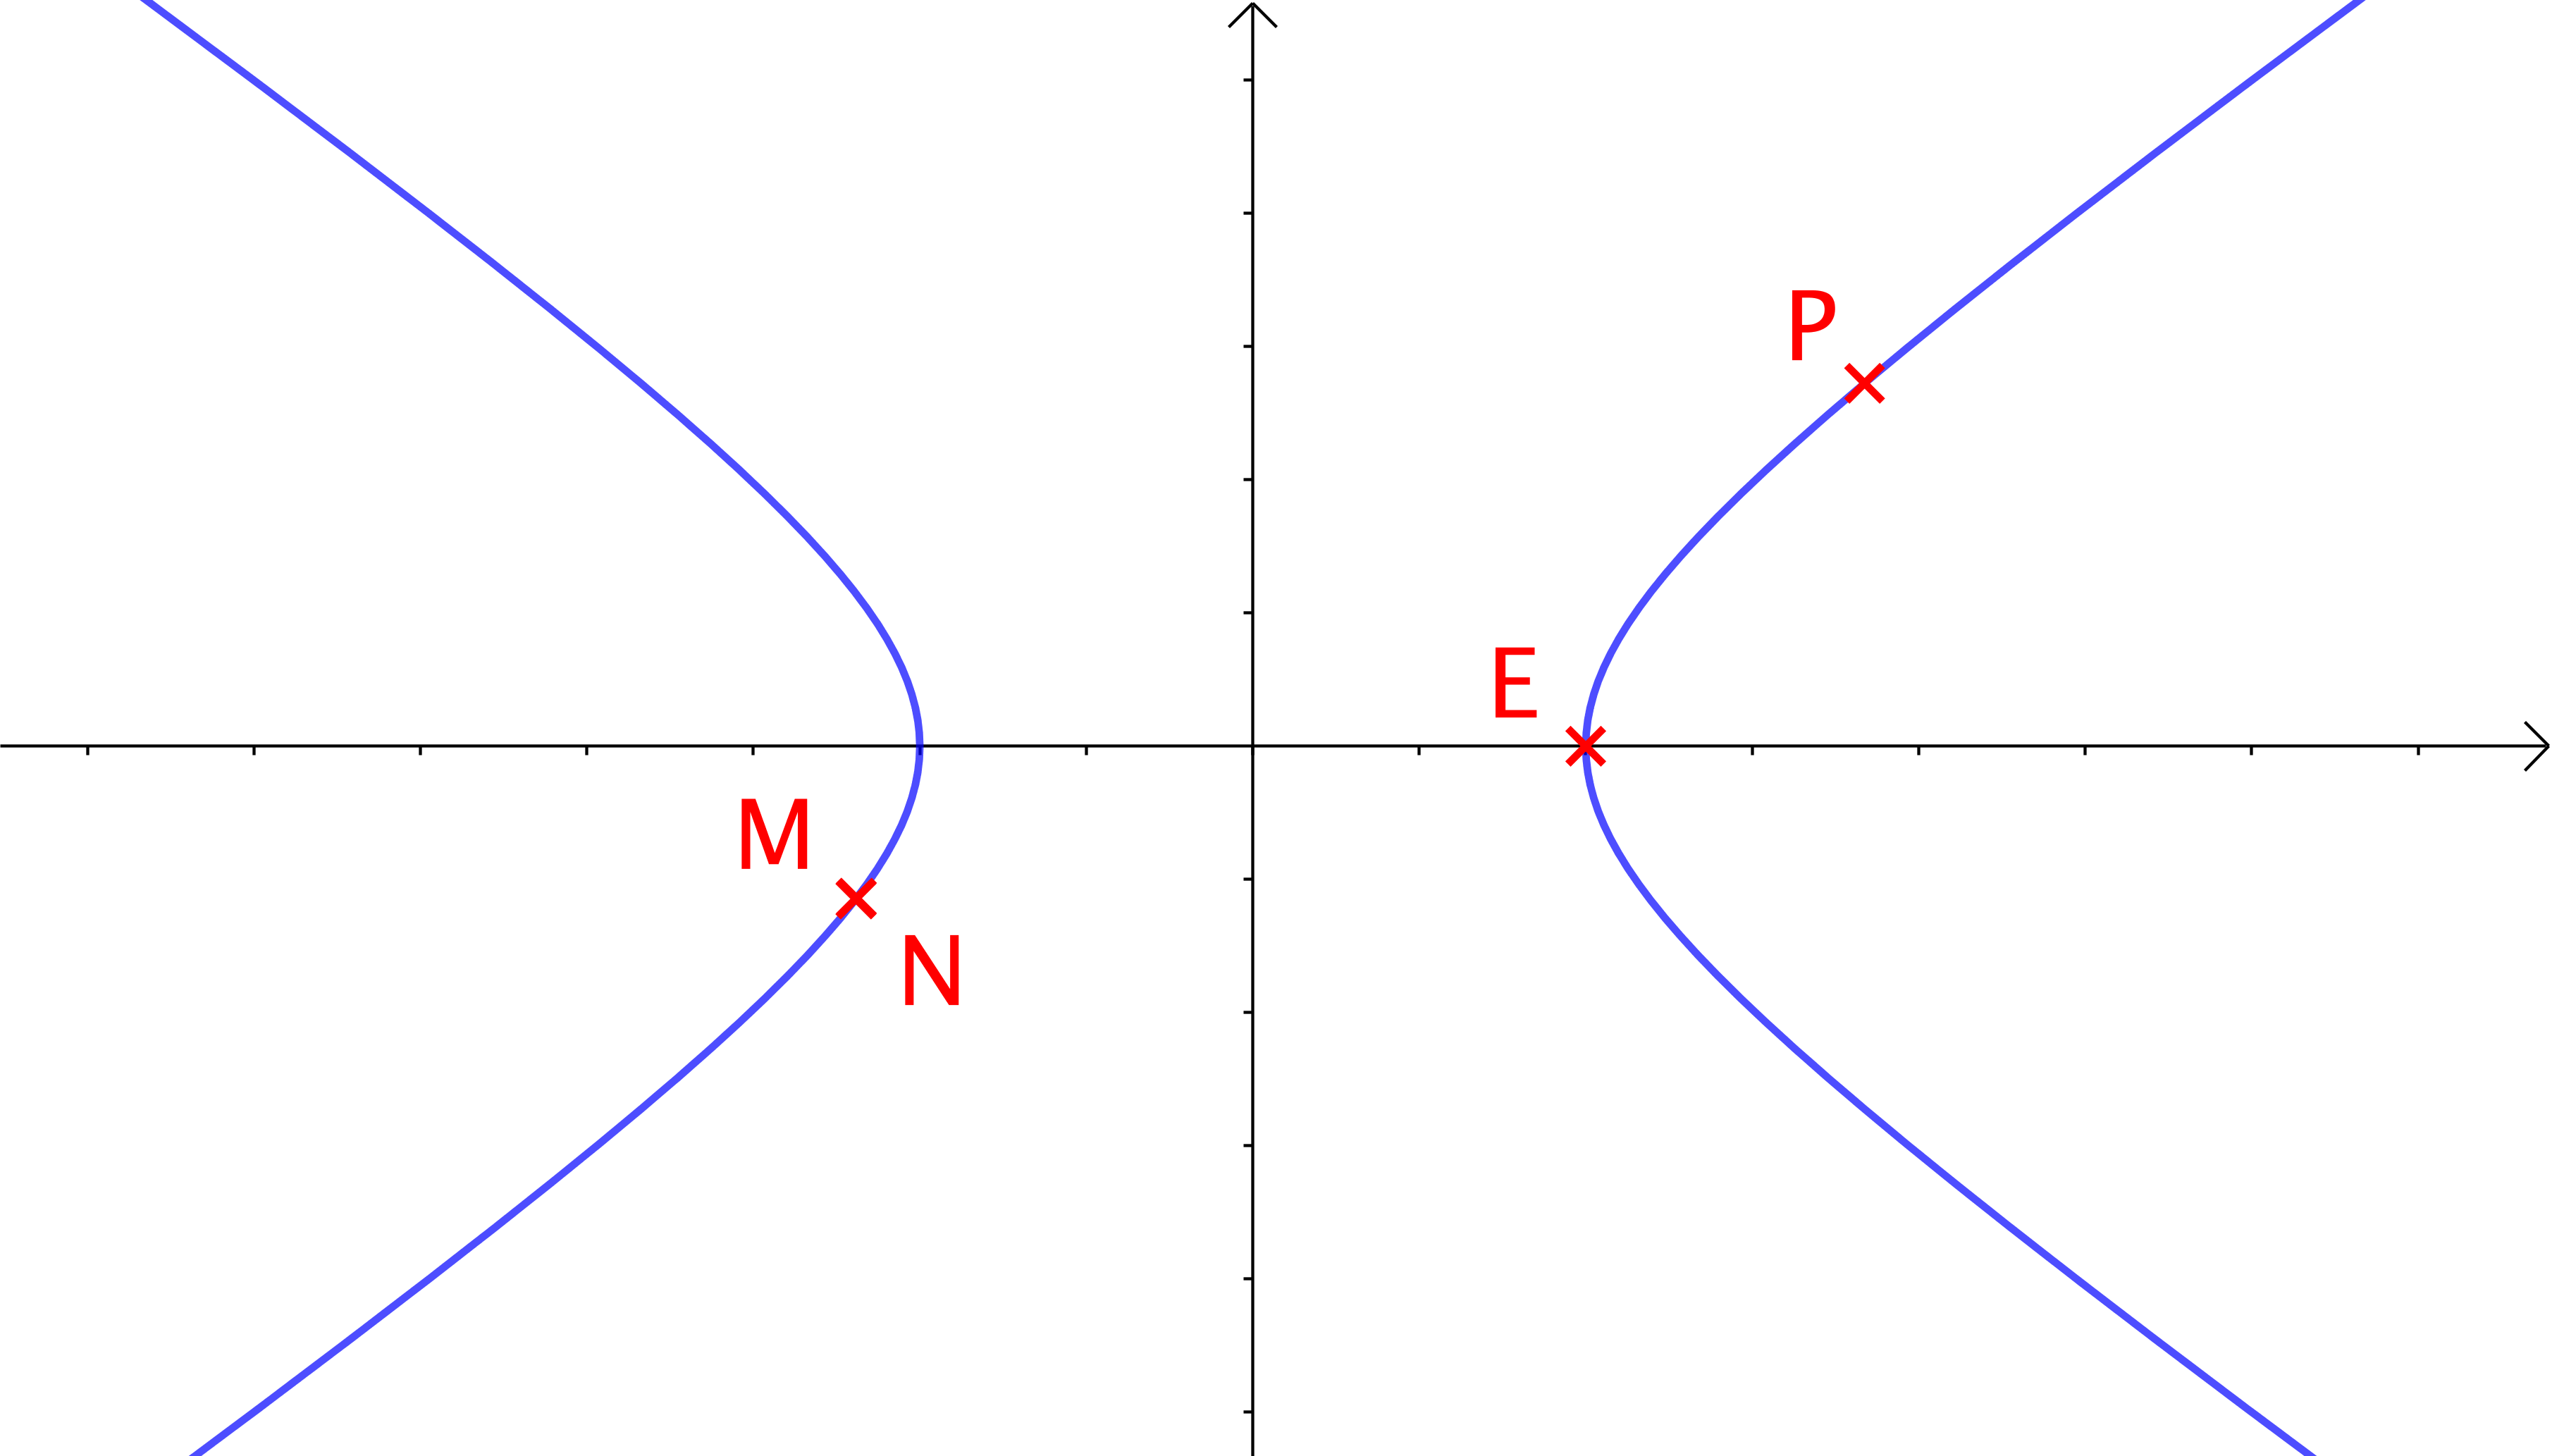
\includegraphics[scale = .5]{exo-spe-math-bac-s-juin-2018/geometry-is-the-queen/same-points.png}}
\end{multicols}


\bigskip
	

Les graphiques précédents suggèrent
\footnote{
	Le lieu de téléchargement de ce document contient un fichier GeoGebra \texttt{base-tool.ggb} manipulable dynamiquement pour vérifier combien il est aisé de conjecturer la construction géométrique.
}
un procédé géométrique simple pour construire $P$.

\begin{enumerate}
	\item Si $M \neq N$ et $x_M \neq x_N$ alors on construit la parallèle à $(MN)$ passant par $E$ . Le point $P$ est le second point d'intersection de cette parallèle avec $\setgeo{H}$ \emph{(notons qu'une droite coupe $\setgeo{H}$ en au plus deux points)}.


	\item Si $M \neq N$ et $x_M = x_N$ alors $P = E$ . Notons au passage que l'on peut voir ceci comme un cas limite du précédent avec un point d'intersection \squote{double}.


	\item Si $M = N$ on procède comme ci-dessus mais avec la parallèle de la tangente à $\setgeo{H}$ au point $M$ .
\end{enumerate}


Dans les graphiques suivants, nous avons tracé les droites utilisées par le procédé géométrique conjecturé à l'instant.


\medskip


\begin{multicols}{2}
	\center
	
	\fbox{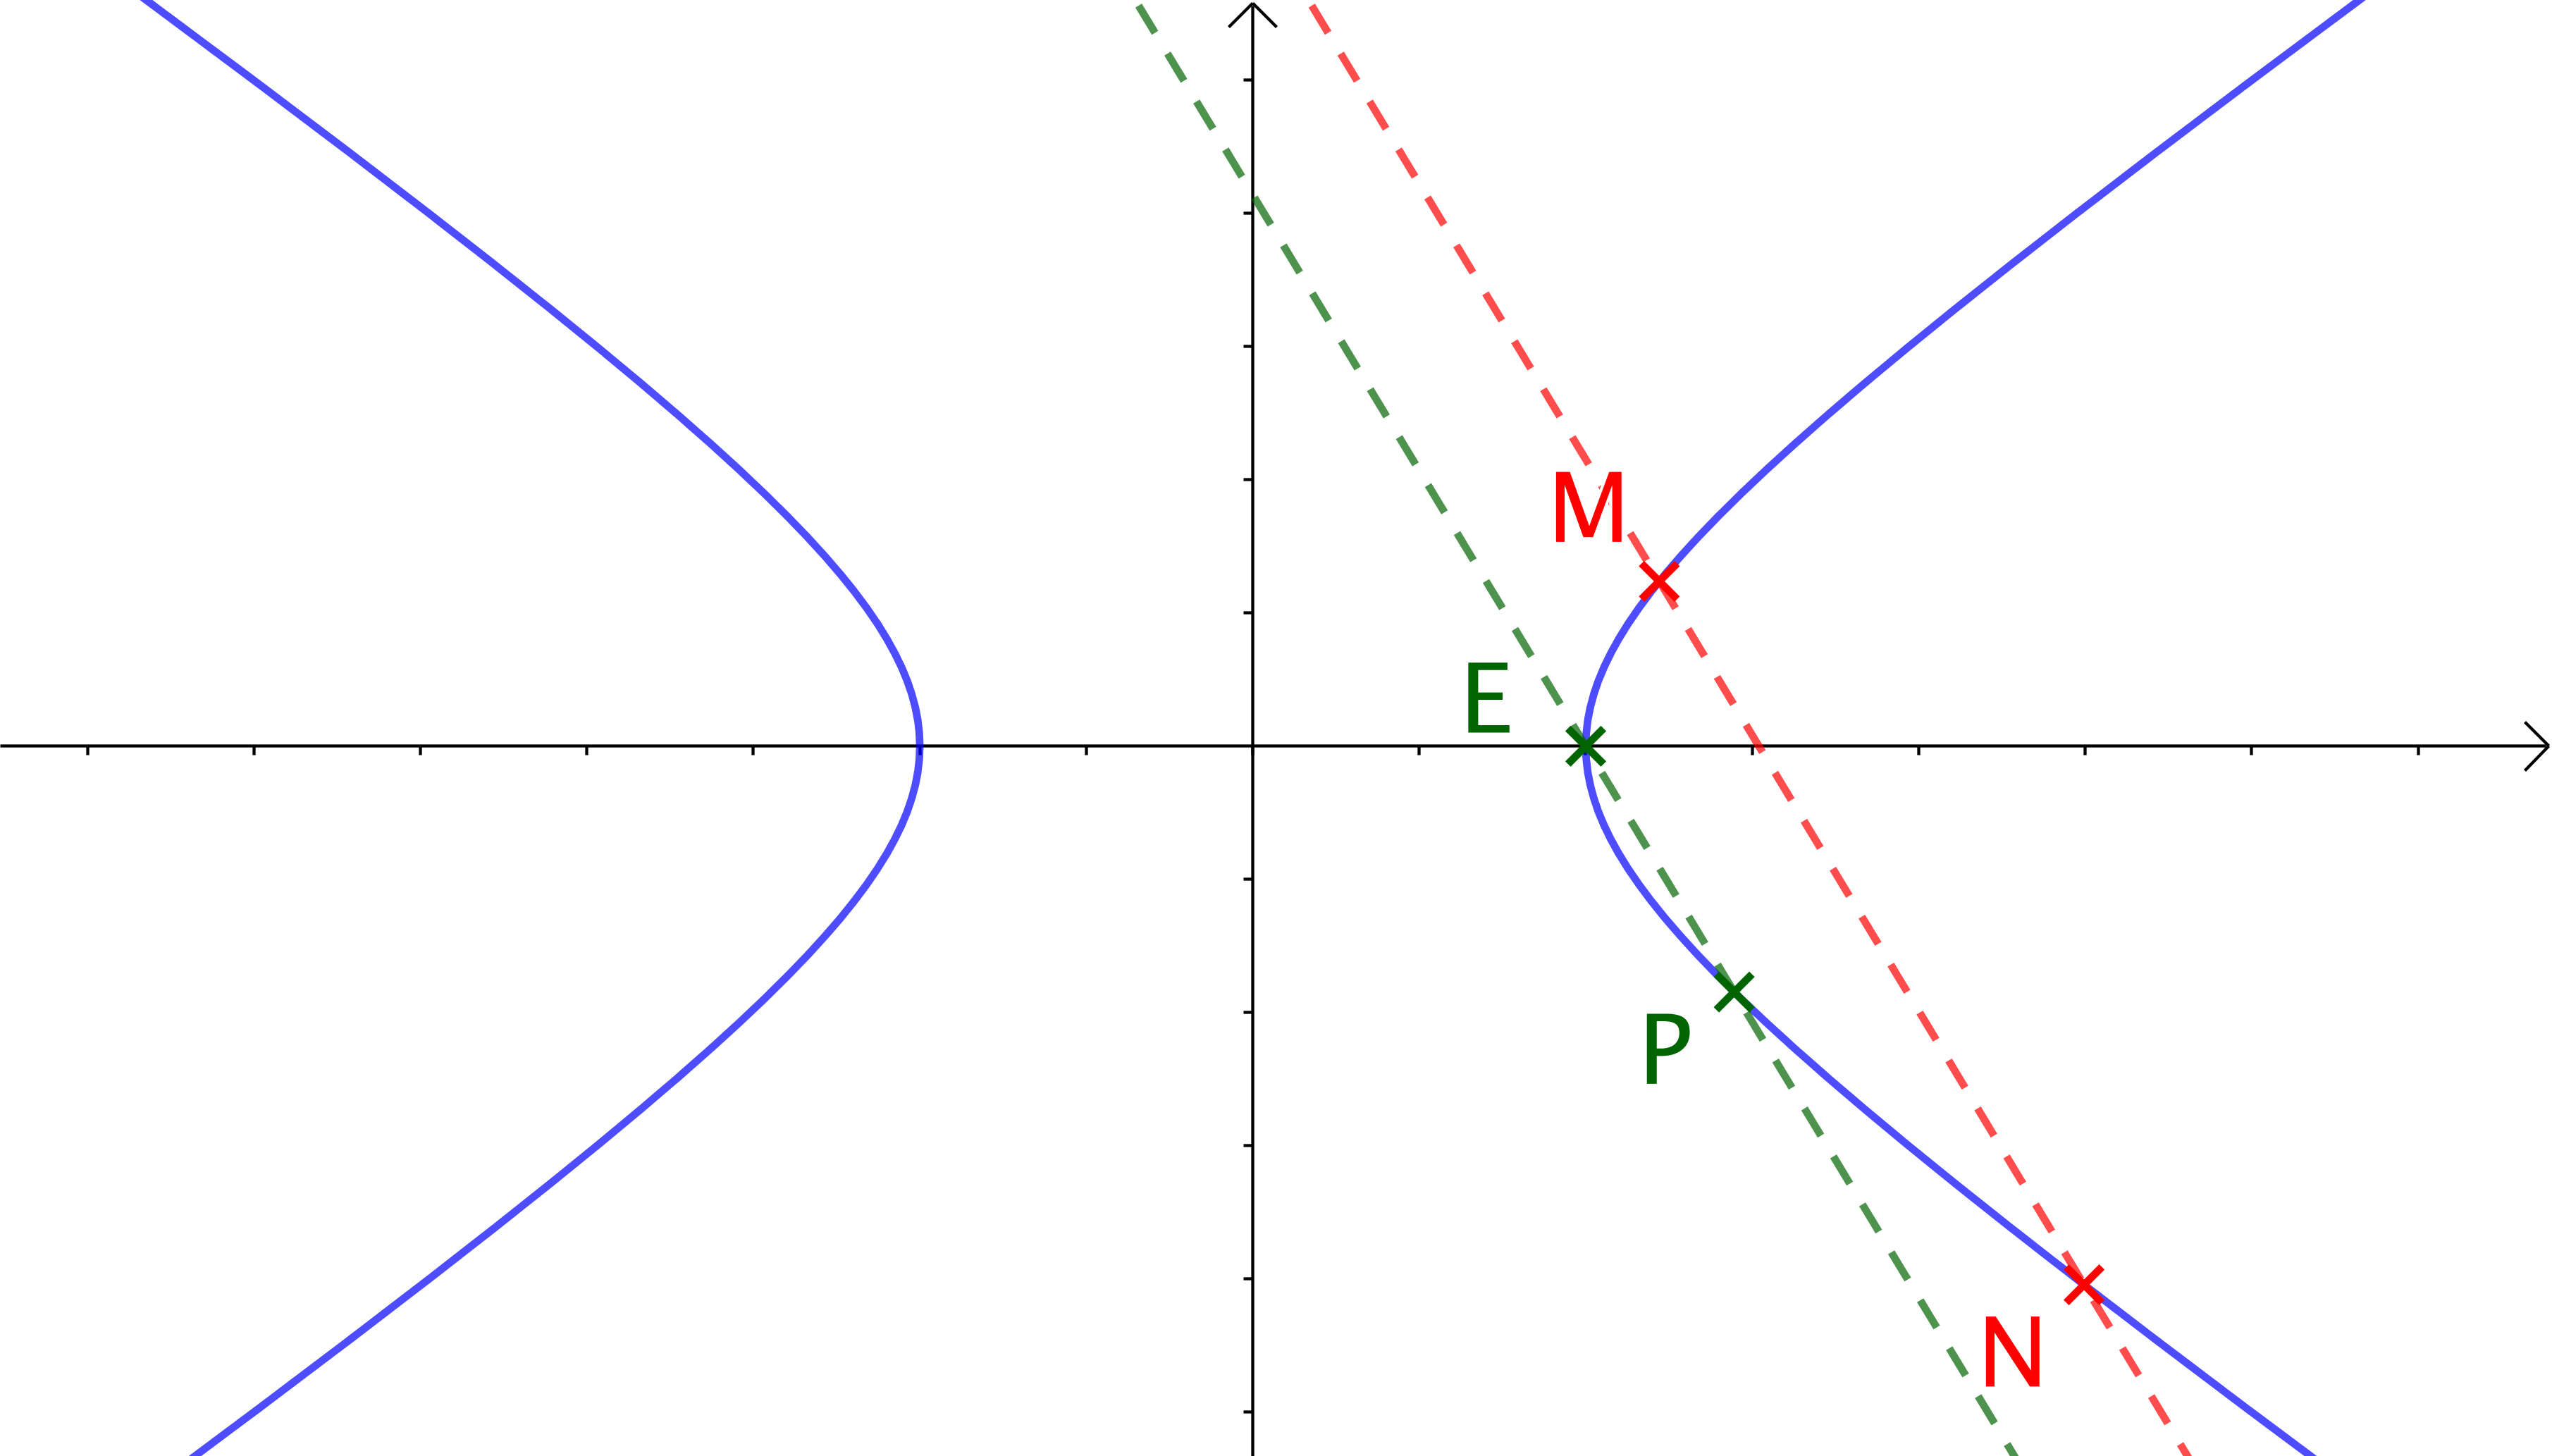
\includegraphics[scale = .5]{exo-spe-math-bac-s-juin-2018/geometry-is-the-queen/oblic-1-with-lines.png}}
	
	\bigskip
	
	\fbox{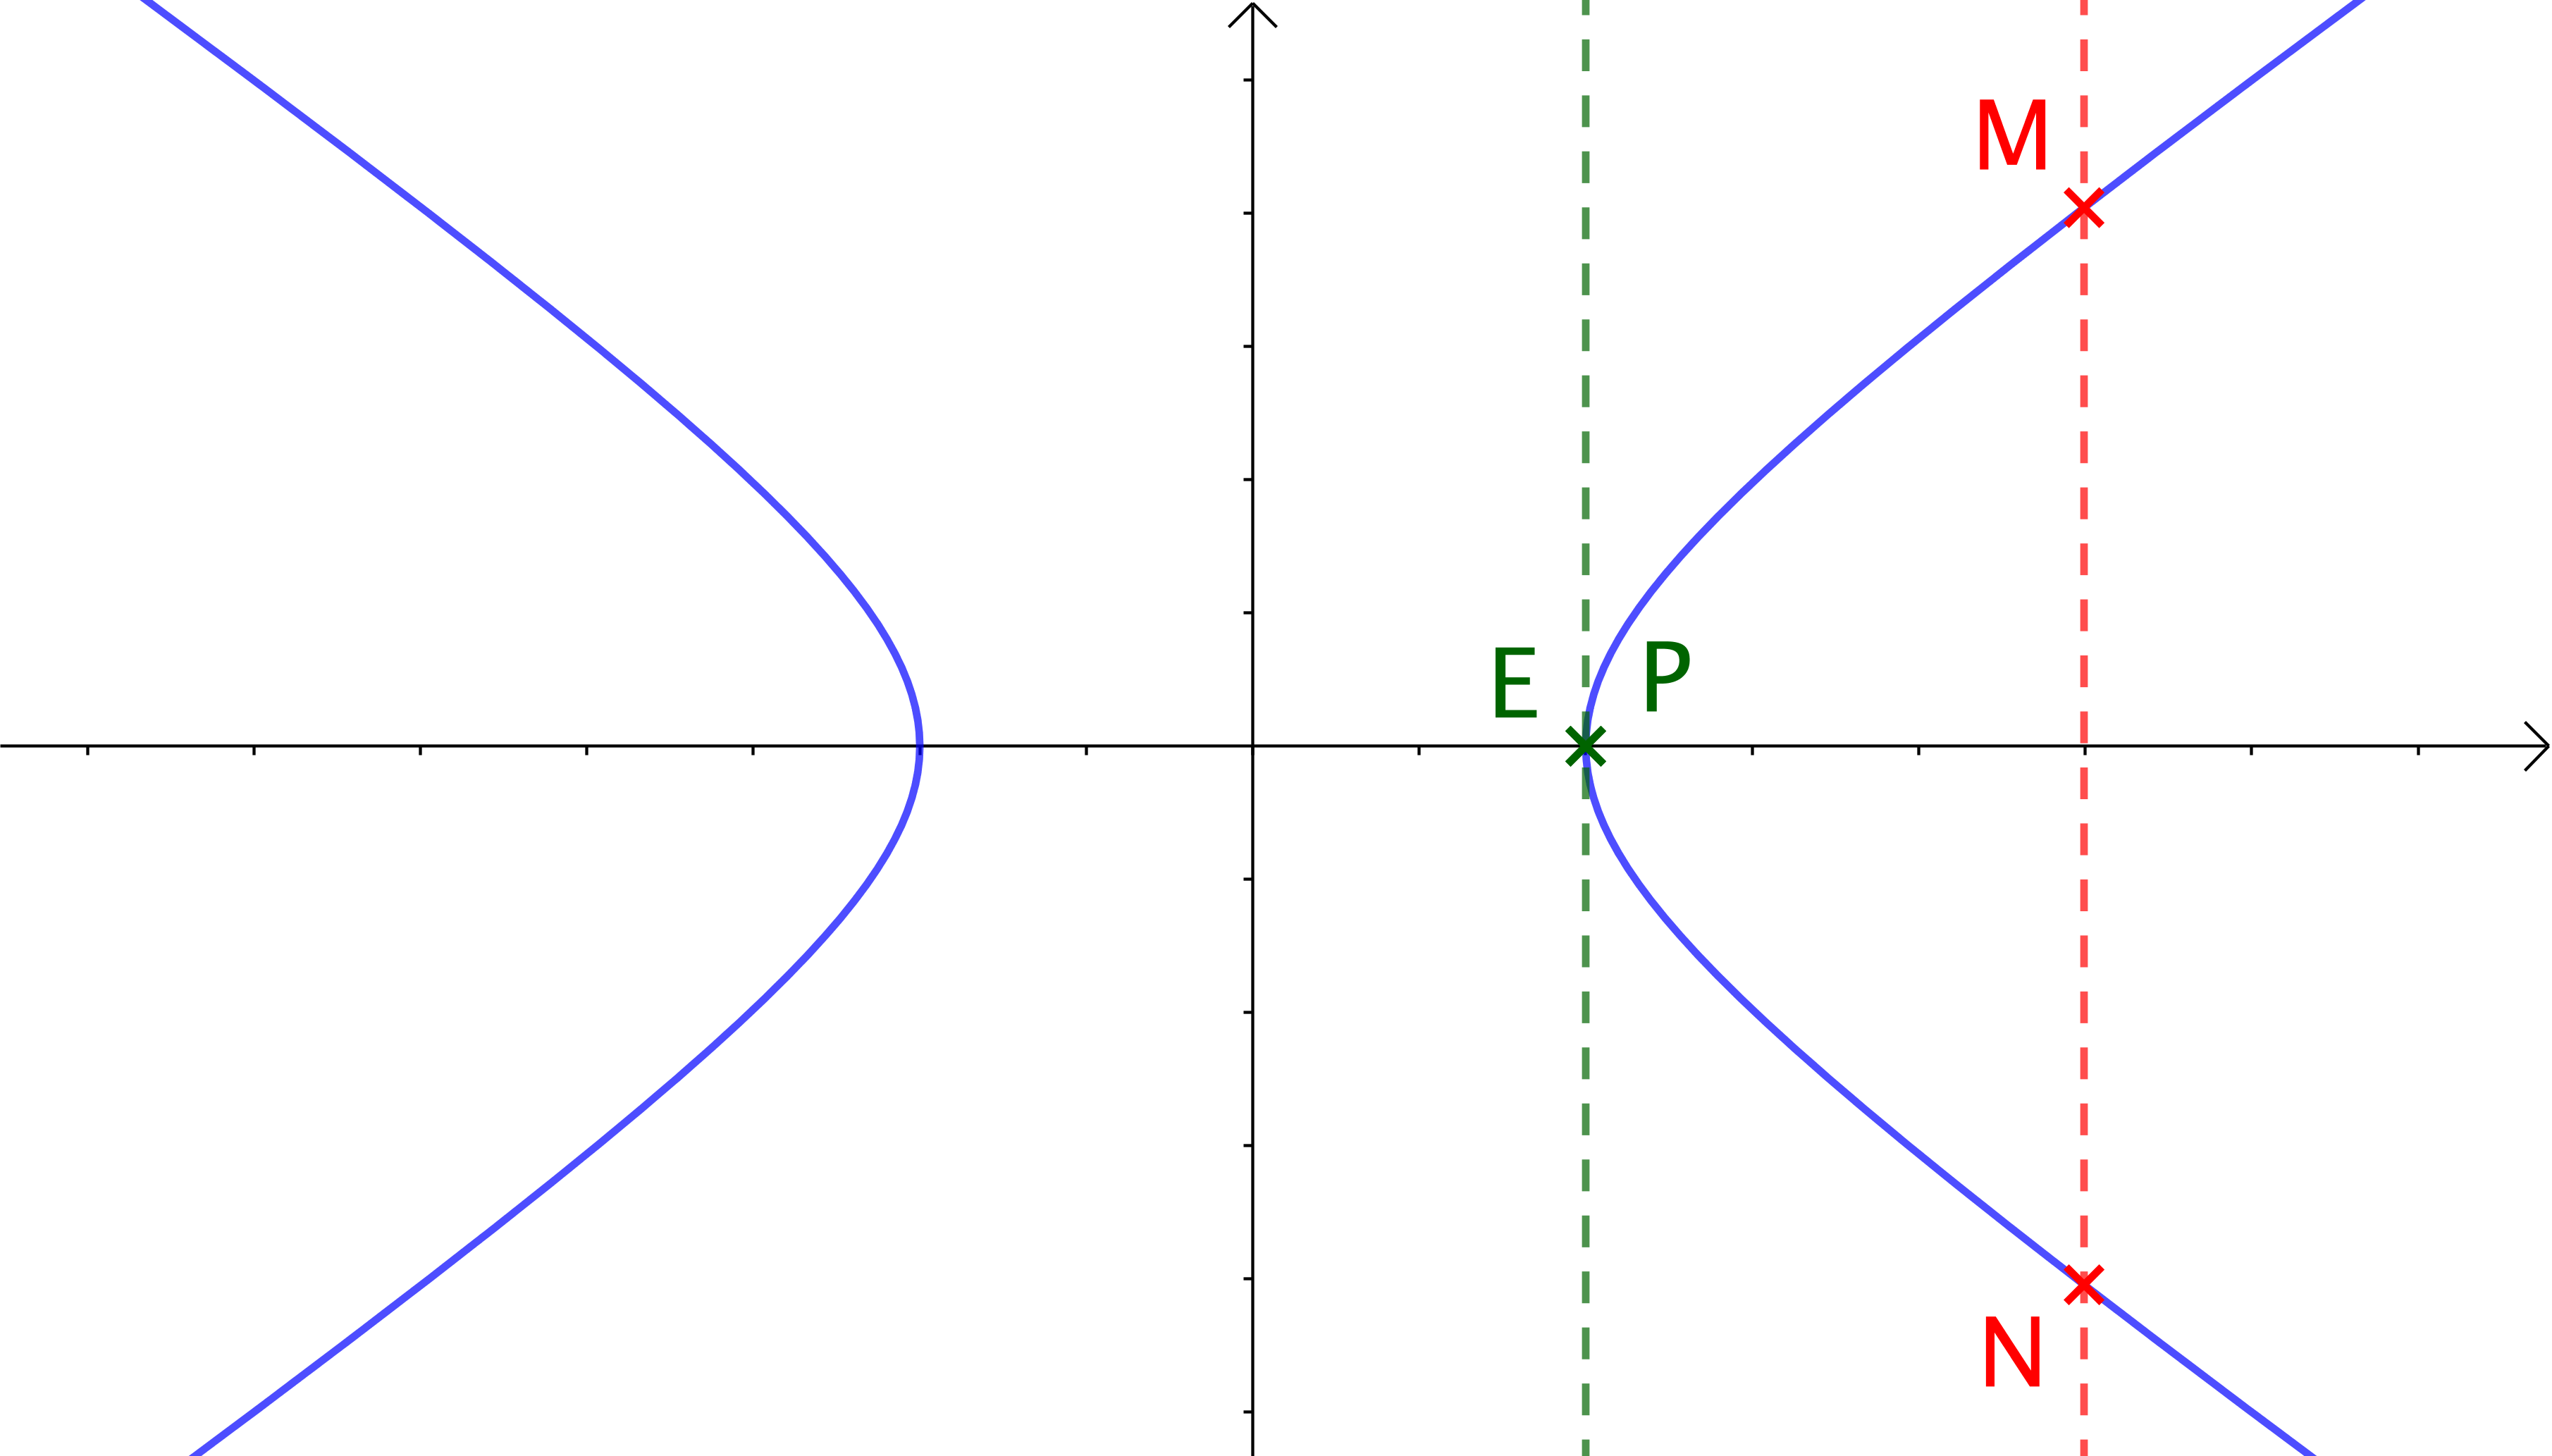
\includegraphics[scale = .5]{exo-spe-math-bac-s-juin-2018/geometry-is-the-queen/vertical-case-with-lines.png}}

	\columnbreak
	
	\fbox{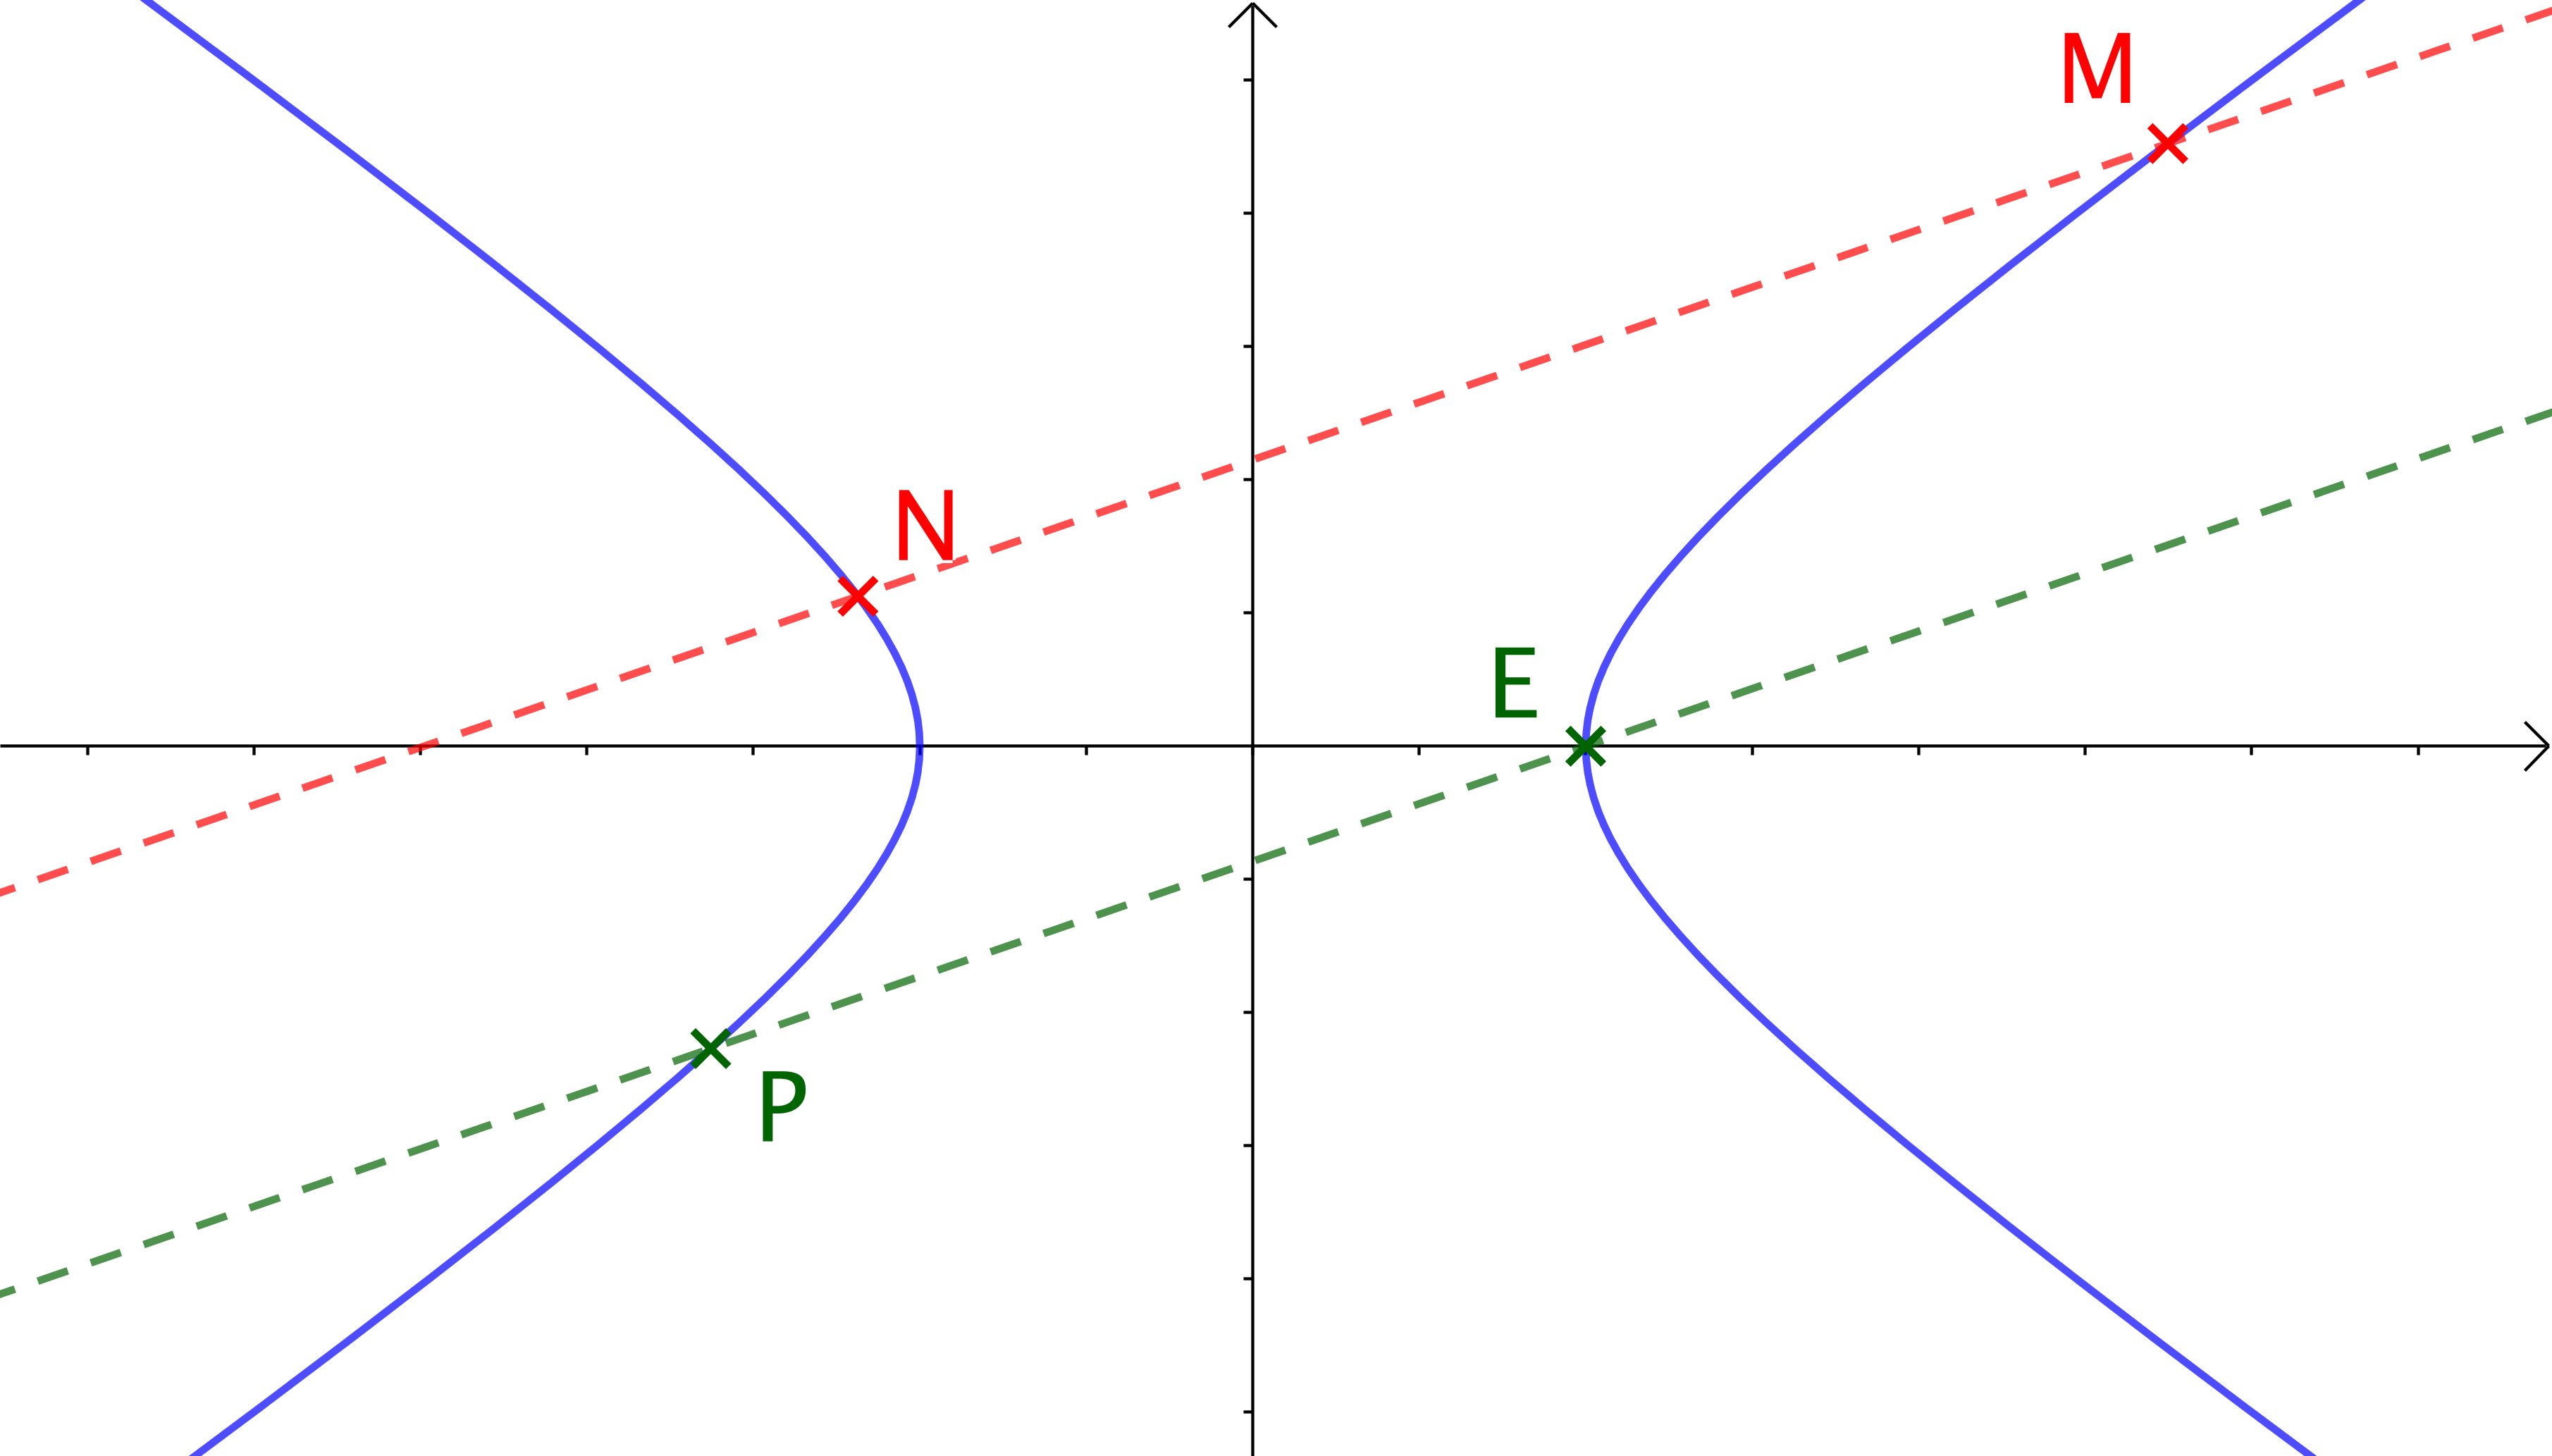
\includegraphics[scale = .5]{exo-spe-math-bac-s-juin-2018/geometry-is-the-queen/oblic-2-with-lines.png}}
	
	\bigskip

	\fbox{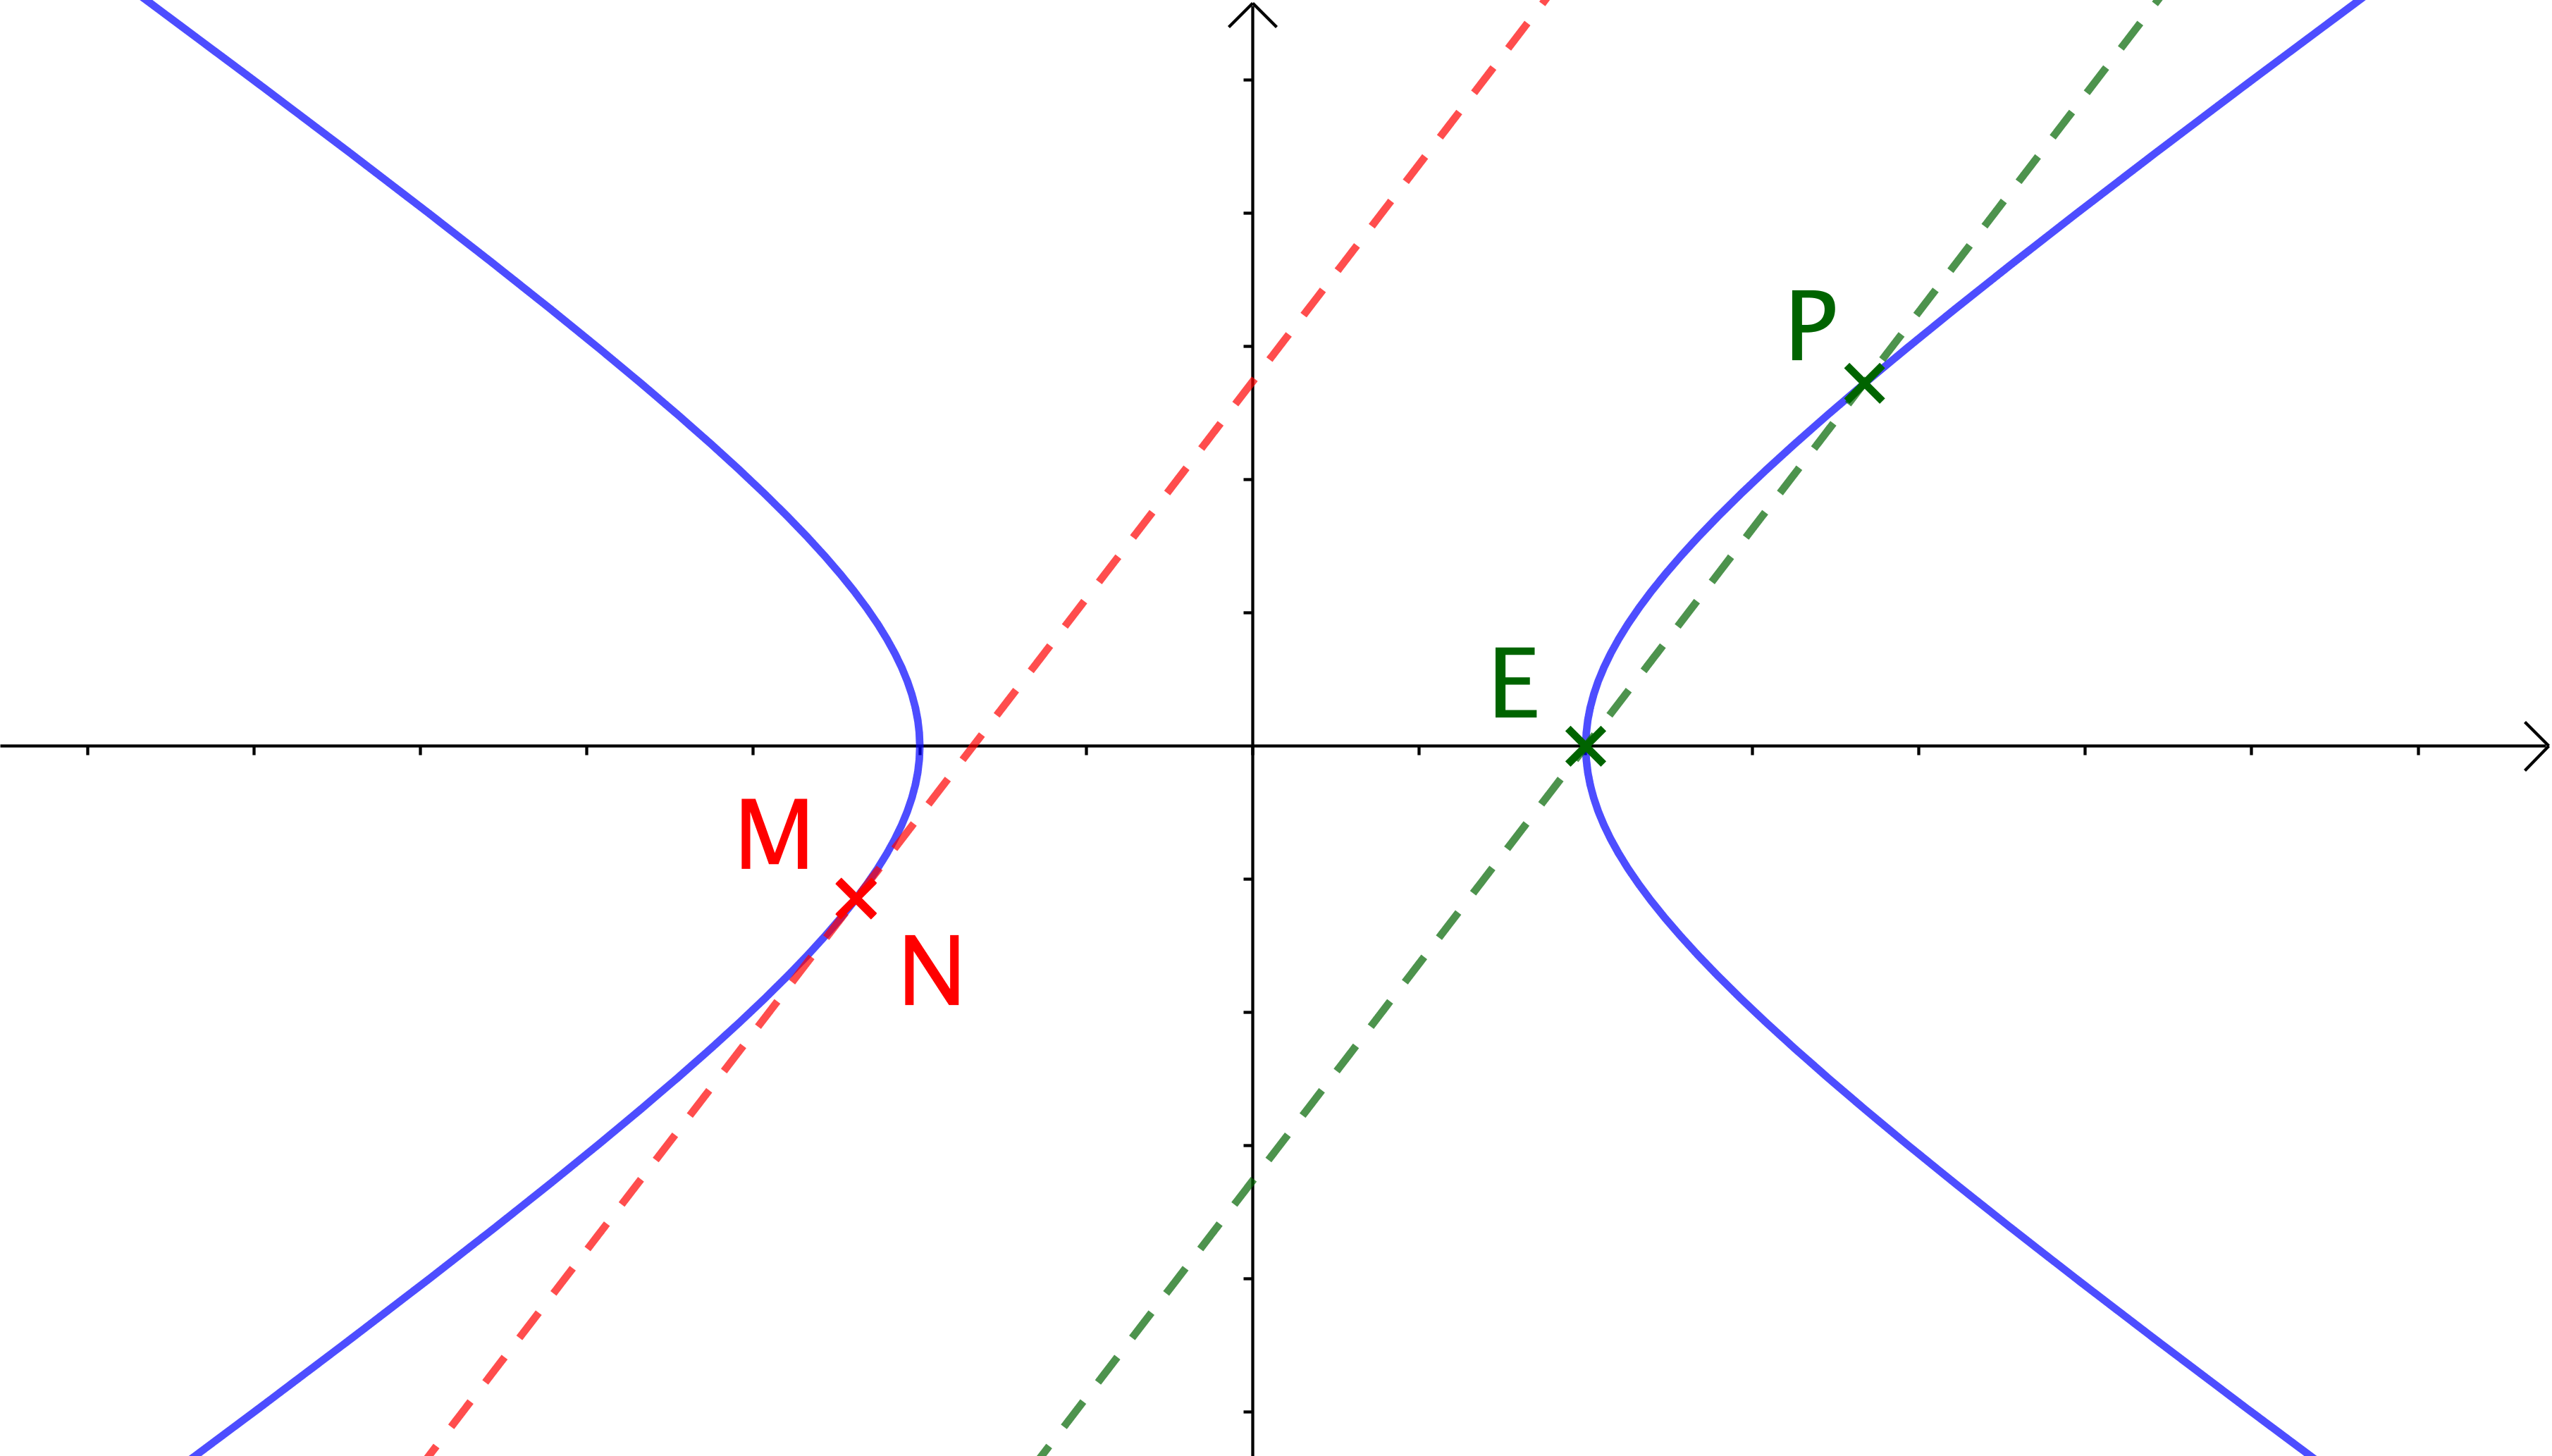
\includegraphics[scale = .5]{exo-spe-math-bac-s-juin-2018/geometry-is-the-queen/same-points-with-lines.png}}
\end{multicols}


\bigskip

Prouvons la validité de notre conjecture. Nous confondrons les points avec les vecteurs utilisés pour définir la loi $\star$ .

\begin{enumerate}
	\item Supposons que $M \neq N$ avec $x_M \neq x_N$ .
	
	\smallskip
	
	\noindent
	Nous devons juste vérifier que $(EP)$ et $(MN)$ sont parallèles puisque l'on sait que $P \neq E$ \textit{(voir le point suivant si besoin)}. Ce qui suit est quelque peu brutal \textit{(on pourrait faire appel à un logiciel de calcul formel qui ici peut être utilisé en toute confiance)}.
	
	\smallskip
	
	\noindent
	$\det\left ( \vect{EP} ; \vect{MN} \right)
	=
	\left|\begin{NiceArray}{cc} 
	  x'' - 1 & x' - x \\ 
	  y''     & y' - y
	\end{NiceArray}\right|$
	
	\noindent
	$\phantom{\det\left ( \vect{EP} ; \vect{MN} \right)}
	=
	(x'' - 1)(y' - y) -  y'' (x' - x)$
	
	\noindent
	$\phantom{\det\left ( \vect{EP} ; \vect{MN} \right)}
	=
	(x x' + 8 y y' - 1)(y' - y) -  (y x' + x y') (x' - x)$
	
	\noindent
	$\phantom{\det\left ( \vect{EP} ; \vect{MN} \right)}
	=
	x x' y' + 8 y y'^2 - y' - x x' y - 8 y^2 y' + y
	- 
	y x'^2 - x x' y' + y x x' + x^2 y'$
	
	\noindent
	$\phantom{\det\left ( \vect{EP} ; \vect{MN} \right)}
	=
	8 y y'^2 - y' - 8 y^2 y' + y
	- 
	y x'^2 + x^2 y'$
	
	\smallskip
	
	\noindent
	Réordonnons les termes en nous souvenant que $x^2 - 8 y^2 = 1$ et $x'^2 - 8 y'^2 = 1$ .

	\smallskip
	
	\noindent
	${\det\left ( \vect{EP} ; \vect{MN} \right)}
	=
	x^2 y' - 8 y^2 y'
	- y x'^2 + 8 y y'^2
	- y' + y$
	
	\noindent
	$\phantom{\det\left ( \vect{EP} ; \vect{MN} \right)}
	=
	(x^2 - 8 y^2)y'
	- y(x'^2 - 8 y'^2)
	- y' + y$
	
	\noindent
	$\phantom{\det\left ( \vect{EP} ; \vect{MN} \right)}
	=
	y'
	- y
	- y' + y$
	
	\noindent
	$\phantom{\det\left ( \vect{EP} ; \vect{MN} \right)}
	=
	0$
	
	\smallskip
	
	\noindent
	Nous avons bien vérifié le parallélisme des droites $(EP)$ et $(MN)$ .

% --------------- %

	\medskip
	\item Supposons que $M \neq N$ avec $x_M = x_N$ .
	
	\smallskip
	
	\noindent
	Dans ce cas, comme $x_M = x_N$ et $y_M = -y_N$ , nous avons
	$x_M x_N + 8 y_M y_N = x_M^2 - 8 y_M^2 = 1$
	et
	$y_M x_N + x_M y_N = 0$ .
	Ceci justifie que $P = E$ .

% --------------- %

	\medskip
	\item Supposons que $M = N$ .
	
	\smallskip
	
	\noindent
	Notant $F(X ; Y) = X^2 - 8 Y^2 - 1$ , la tangente à $\setproba{H} : F(X ; Y) = 0$ en $M$ admet pour vecteur directeur
	$\vect{u} \begin{pmatrix} 
	  - \pder{F}{Y}{1}(x ; y)    \\ 
	  \pder{F}{X}{1}(x ; y) 
	\end{pmatrix}$
	c'est à dire
	$\vect{u} \begin{pmatrix} 
	  16y    \\ 
	  2x 
	\end{pmatrix}$
	sous la condition $(x ; y) \neq (0 ; 0)$ qui est vérifiée par tout point de notre hyperbole $\setgeo{H}$. 
	
	
	\noindent
	Comme de plus $x'' = x^2 + 8y^2 = 16y^2 + 1$ et $y'' = 2xy$, nous avons
	$\vect{EP} \begin{pmatrix} 
	  16y^2    \\ 
	  2xy
	\end{pmatrix}$
	d'où
	$\vect{EP} = y \vect{u}$.
	Ceci permet de conclure.
\end{enumerate}



\bigskip

\textbf{Remarque.} Pour ceux qui connaissent la loi de groupe des courbes elliptiques, notons que ce qui précède peut être un point d'entrée naturel, et humainement calculable, vers celle-ci \textit{(indiquons qu'il existe un moyen naturel, mais d'une très grande technicité, de tomber sur cette fameuse loi de groupe qui est trop souvent donnée violemment sans plus d'explications sur la raison du procédé géométrique qui lui est associé)}.


\end{document}
